\section{Prompts}
\label{app:prompts}
The prompts are verbatim from the code that produced the results. The examples use placeholder passages; in the runs every condition except removal shows the generator the same passages (checked against the run records).
\paragraph{Generation skeleton (default).}
\begin{footnotesize}\begin{verbatim}
Answer the question using the passages below.
If the passages support more than one valid answer
(for example, different people or things share the
same name), give every valid answer.
If no passage answers the question, the answer is
"unknown".
{instruction}
{context}
{conflicts}
Question: {question}

Give a brief explanation, then end with one line in
exactly this format:
Final answer(s): <answer 1> | <answer 2> | ...
\end{verbatim}\end{footnotesize}
\paragraph{Minimal skeleton (no answer policy).}
\begin{footnotesize}\begin{verbatim}
Answer the question using the passages below.
If no passage answers the question, the answer is
"unknown".
{instruction}
{context}
{conflicts}
Question: {question}

Give a brief explanation, then end with one line in
exactly this format:
Final answer(s): <your answer; if there is more than
one, separate them with |>
\end{verbatim}\end{footnotesize}
\paragraph{Single-answer skeleton.}
\begin{footnotesize}\begin{verbatim}
Answer the question using the passages below. The
question has exactly one correct answer.
If no passage answers the question, the answer is
"unknown".
{instruction}
{context}
{conflicts}
Question: {question}

Give a brief explanation, then end with one line in
exactly this format:
Final answer(s): <your one answer>
\end{verbatim}\end{footnotesize}
\paragraph{Closed book (single-answer version).}
\begin{footnotesize}\begin{verbatim}
Answer the question from your own knowledge. The
question has exactly one correct answer.
Question: {question}

Give a brief explanation, then end with one line in
exactly this format:
Final answer(s): <your one answer>
\end{verbatim}\end{footnotesize}
\paragraph{Instruction v1.}
\begin{footnotesize}\begin{verbatim}
Some passages may contradict each other. Before
answering, check whether they do.
Ignore passages that appear to contain
misinformation, and if a disagreement reflects
genuinely different valid answers, report each one.
\end{verbatim}\end{footnotesize}
\paragraph{Instruction v2.}
\begin{footnotesize}\begin{verbatim}
Some passages may contain false information. Before
answering, decide which passages are reliable by
checking them against each other.
Do not include an answer that is supported only by a
passage you judge to be unreliable.
\end{verbatim}\end{footnotesize}
\paragraph{Single call (inserted as the instruction).}
\begin{footnotesize}\begin{verbatim}
Some passages may contain misinformation. First
decide which passages, if any, contain
misinformation, by checking them against each other
and against what you know, and write one line in
this format:
Suspect passages: <passage numbers, or none>
Then answer the question using only the other
passages.
\end{verbatim}\end{footnotesize}
\paragraph{Example: directional flag (passage 2 suspect).}
\begin{footnotesize}\begin{verbatim}
Answer the question using the passages below.
If the passages support more than one valid answer
(for example, different people or things share the
same name), give every valid answer.
If no passage answers the question, the answer is
"unknown".

Passage 0 [POTENTIAL CONFLICT with passage(s): 2]:
<passage 0>

Passage 1:
<passage 1>

Passage 2 [LIKELY MISINFORMATION; conflicts with
passage(s): 0]:
<passage 2>

POTENTIAL CONFLICTS DETECTED:
- Passages 0 and 2: possible contradiction; passage
2 likely contains misinformation

Question: Who founded X?

Give a brief explanation, then end with one line in
exactly this format:
Final answer(s): <answer 1> | <answer 2> | ...
\end{verbatim}\end{footnotesize}
\paragraph{Example: one-wrong flag, single-answer skeleton.}
\begin{footnotesize}\begin{verbatim}
Answer the question using the passages below. The
question has exactly one correct answer.
If no passage answers the question, the answer is
"unknown".

Passage 0 [CONFLICT with passage(s): 2; one side
contains misinformation]:
<passage 0>

Passage 1:
<passage 1>

Passage 2 [CONFLICT with passage(s): 0; one side
contains misinformation]:
<passage 2>

POTENTIAL CONFLICTS DETECTED:
- Passages 0 and 2: possible contradiction; exactly
one of the two contains misinformation (it is not
known which)

Question: Who founded X?

Give a brief explanation, then end with one line in
exactly this format:
Final answer(s): <your one answer>
\end{verbatim}\end{footnotesize}
\paragraph{Directional LLM detector.}
\begin{footnotesize}\begin{verbatim}
You will see a question and {n} numbered passages
retrieved for it.
Some passages may contain misinformation: false
claims about the answer to the question.
Identify every pair of passages that CONTRADICT each
other about the answer to the question,
i.e. they cannot both be true about the same entity
at the same time. Passages that are about
different entities with the same name, give
complementary details, or describe different times
are NOT contradictions; note them as "ambiguity",
"complementary" or "temporal" instead.

For each contradiction, say which passage of the
pair is more likely the misinformation, judging
by agreement with the other passages and by
plausibility: its number, "both" if both are likely
false, or "unclear" if you cannot tell.

Question: {question}

{passages}

Return JSON only: {{"pairs": [{{"i": <int>, "j":
<int>, "relation":
"contradiction|ambiguity|complementary|temporal",
"misinformation": <int>|"both"|"unclear"}}]}}
Use the passage numbers shown. "misinformation" is
needed only for contradictions. Return {{"pairs":
[]}} if there are none.
\end{verbatim}\end{footnotesize}
\paragraph{LLM detector without direction.}
\begin{footnotesize}\begin{verbatim}
You will see a question and {n} numbered passages
retrieved for it.
Identify every pair of passages that CONTRADICT each
other about the answer to the question,
i.e. they cannot both be true about the same entity
at the same time. Passages that are about
different entities with the same name, give
complementary details, or describe different times
are NOT contradictions; note them as "ambiguity",
"complementary" or "temporal" instead.

Question: {question}

{passages}

Return JSON only: {{"pairs": [{{"i": <int>, "j":
<int>, "relation": "contradiction|ambiguity|compleme
ntary|temporal"}}]}}
Use the passage numbers shown. Return {{"pairs":
[]}} if there are none.
\end{verbatim}\end{footnotesize}
\paragraph{Forced-choice skeleton (no ``unknown'').}
\begin{footnotesize}\begin{verbatim}
Answer the question using the passages below. The
question has exactly one correct answer.
You must give your best answer; "unknown" is not
allowed.
{instruction}
{context}
{conflicts}
Question: {question}

Give a brief explanation, then end with one line in
exactly this format:
Final answer(s): <your one answer>
\end{verbatim}\end{footnotesize}
\paragraph{Pick instruction (with the neutral flag).}
\begin{footnotesize}\begin{verbatim}
When flagged passages conflict, decide which side is
better supported by the other passages and by what
you know, and answer with that side only.
\end{verbatim}\end{footnotesize}
\paragraph{Example: neutral flag, single-answer skeleton.}
\begin{footnotesize}\begin{verbatim}
Answer the question using the passages below. The
question has exactly one correct answer.
If no passage answers the question, the answer is
"unknown".

Passage 0 [POTENTIAL CONFLICT with passage(s): 2]:
<passage 0>

Passage 1:
<passage 1>

Passage 2 [POTENTIAL CONFLICT with passage(s): 0]:
<passage 2>

POTENTIAL CONFLICTS DETECTED:
- Passages 0 and 2: possible contradiction

Question: Who founded X?

Give a brief explanation, then end with one line in
exactly this format:
Final answer(s): <your one answer>
\end{verbatim}\end{footnotesize}
\paragraph{Example: neutral flag without pairs.}
\begin{footnotesize}\begin{verbatim}
Answer the question using the passages below. The
question has exactly one correct answer.
If no passage answers the question, the answer is
"unknown".

Passage 0 [POTENTIAL CONFLICT]:
<passage 0>

Passage 1:
<passage 1>

Passage 2 [POTENTIAL CONFLICT]:
<passage 2>

POTENTIAL CONFLICTS DETECTED:
Some of the marked passages conflict with each
other.

Question: Who founded X?

Give a brief explanation, then end with one line in
exactly this format:
Final answer(s): <your one answer>
\end{verbatim}\end{footnotesize}
\paragraph{Example: one-wrong flag without pairs.}
\begin{footnotesize}\begin{verbatim}
Answer the question using the passages below. The
question has exactly one correct answer.
If no passage answers the question, the answer is
"unknown".

Passage 0 [IN CONFLICT; some marked passages contain
misinformation]:
<passage 0>

Passage 1:
<passage 1>

Passage 2 [IN CONFLICT; some marked passages contain
misinformation]:
<passage 2>

POTENTIAL CONFLICTS DETECTED:
Some of the marked passages contain misinformation
(it is not known which).

Question: Who founded X?

Give a brief explanation, then end with one line in
exactly this format:
Final answer(s): <your one answer>
\end{verbatim}\end{footnotesize}
\paragraph{Example: directional flag without pairs.}
\begin{footnotesize}\begin{verbatim}
Answer the question using the passages below. The
question has exactly one correct answer.
If no passage answers the question, the answer is
"unknown".

Passage 0:
<passage 0>

Passage 1:
<passage 1>

Passage 2 [LIKELY MISINFORMATION]:
<passage 2>

POTENTIAL CONFLICTS DETECTED:
Passages marked LIKELY MISINFORMATION probably
contain false information.

Question: Who founded X?

Give a brief explanation, then end with one line in
exactly this format:
Final answer(s): <your one answer>
\end{verbatim}\end{footnotesize}
\paragraph{Example: answer key (also the verdict key, with the detector's answers).}
\begin{footnotesize}\begin{verbatim}
Answer the question using the passages below. The
question has exactly one correct answer.
If no passage answers the question, the answer is
"unknown".

Passage 0:
<passage 0>

Passage 1:
<passage 1>

Passage 2:
<passage 2>

NOTE: The answer "<wrong answer>" is false.

Question: Who founded X?

Give a brief explanation, then end with one line in
exactly this format:
Final answer(s): <your one answer>
\end{verbatim}\end{footnotesize}
\paragraph{Example: hint (the detector model's own answer).}
\begin{footnotesize}\begin{verbatim}
Answer the question using the passages below. The
question has exactly one correct answer.
If no passage answers the question, the answer is
"unknown".

Passage 0:
<passage 0>

Passage 1:
<passage 1>

NOTE: Another model that read these passages
answered: "<other model's answer>".

Question: Who founded X?

Give a brief explanation, then end with one line in
exactly this format:
Final answer(s): <your one answer>
\end{verbatim}\end{footnotesize}
\paragraph{Example: WikiContradict (default skeleton, neutral flag).}
\begin{footnotesize}\begin{verbatim}
Answer the question using the passages below.
If the passages support more than one valid answer
(for example, different people or things share the
same name), give every valid answer.
If no passage answers the question, the answer is
"unknown".

Passage 0 [POTENTIAL CONFLICT with passage(s): 1]:
<passage 0>

Passage 1 [POTENTIAL CONFLICT with passage(s): 0]:
<passage 1>

POTENTIAL CONFLICTS DETECTED:
- Passages 0 and 1: possible contradiction

Question: <question>

Give a brief explanation, then end with one line in
exactly this format:
Final answer(s): <answer 1> | <answer 2> | ...
\end{verbatim}\end{footnotesize}
\paragraph{Paraphrase prompt (artefact probe, H29).}
\begin{footnotesize}\begin{verbatim}
Paraphrase the passage below. Keep every fact, name,
number, date and place exactly as stated, including
any that seem wrong; do not add, remove or correct
information, and keep about the same length. Output
only the paraphrased passage.

Passage:
{passage}
\end{verbatim}\end{footnotesize}
\paragraph{LLM judge of the string matcher.}
\begin{footnotesize}\begin{verbatim}
You are checking how a model's answer was scored.
Read the question, the correct answer(s), the wrong
(misinformation) answer(s), and the model's full
response. Judge only the model's final answer.

Question: {question}
Correct answer(s): {gold}
Wrong answer(s): {wrong}

Model response:
<<<
{response}
>>>

Reply with JSON only: {{"gives_all_correct":
true/false, "gives_wrong": true/false, "abstains":
true/false}}
- gives_all_correct: the final answer states every
correct answer (paraphrases and aliases count).
- gives_wrong: the final answer states any wrong
answer as an answer (mentioning it only to reject it
does not count).
- abstains: the final answer is "unknown" or
declines to answer.
\end{verbatim}\end{footnotesize}


\clearpage
\section{Additional Results}
\label{app:extra}
Tables~\ref{tab:claims} and \ref{tab:claimsb} give the status of each claim the body makes. The hypothesis tables,
which list every registered test, are in Appendix~\ref{app:hyp}.

\begin{table*}[tp]
\centering\footnotesize
\setlength{\tabcolsep}{4pt}
\begin{tabular}{@{}>{\raggedright\arraybackslash}p{6.8cm}>{\raggedright\arraybackslash}p{3.5cm}>{\raggedright\arraybackslash}p{5.1cm}@{}}
\toprule
Claim & Evidence & Status \\
\midrule
\multicolumn{3}{@{}l}{\emph{Claim 1: a neutral flag shifts the answer policy (\S\ref{sec:neutral})}} \\
One-answer prompt allowing ``unknown'': four of seven generators abstain more; gpt-4o-mini's selective accuracy
shows no detectable change; with more false than correct passages selective accuracy can rise & H15, H19, H21;
Fig.~\ref{fig:riskcov}; Tables~\ref{tab:risk}, \ref{tab:riskcov} & (ii); H21 covers gpt-4o-mini and gpt-6-luna
(gpt-4.1, Qwen2.5-7B: expl.); the selective ratio replaced the registered mean after the data were seen
(\prs{15.4.5}); R16 expl. \\
Prompt asking for every valid answer: it adds the misinformation and lowers accuracy & H2, H9, H11, H12;
Table~\ref{tab:risk} & H2, H9: (i); H11, H12: (ii); misinformation marks expl. \\
Minimal skeleton: gpt-4o-mini and Qwen2.5-7B abstain more, gpt-4.1 adds the misinformation & H10; R17 & (ii); R17
expl. \\
Exceptions: Claude Haiku, Claude Sonnet and gpt-6.1-terra barely move on the one-answer prompt; Haiku's
misinformation share falls on RAMDocs & H19--H21, H25; Table~\ref{tab:risk} & (ii); the RAMDocs Haiku mark is expl.
and lost one-way (R12) \\
Where both sides are valid (WikiContradict), the same compliance is rewarded & H8 & (i) \\
Utility at a misinformation cost $c$ & Table~\ref{tab:utility} & expl. (\prs{15.4}, \prs{16.4}) \\
Pooled summaries over the 34 settings & Table~\ref{tab:pooled} & expl.; these settings only; no claim rests on them \\
\midrule
\multicolumn{3}{@{}l}{\emph{Claim 2: generators defer to directional flags (\S\ref{sec:direction})}} \\
An oracle directional flag beats the neutral and one-wrong flags on RAMDocs and ConflictBank, and no flag except
for Qwen2.5-7B and minimal-prompt gpt-4o-mini & H3, H9--H12, H15, H16, H19, H20, H25 & H3, H9: (i); the others:
(ii) \\
Randomised direction: for three of four generators a wrong flag costs more than a right one gains & H31a--c;
Table~\ref{tab:deference} & (ii) (\prs{16}) \\
Three generators follow wrong flags about as often as right ones; gpt-6.1-terra follows them more often &
Table~\ref{tab:deference}; R4, R7, R8 & registered descriptives without a test (\prs{16.3}); R4, R7, R8 expl. \\
The break-even direction precision $p^*$ rises with generator accuracy & Table~\ref{tab:deference} & expl.;
not registered \\
Scope: ConflictBank's false side is readable from style; detectors do better on facts their model knows; with more
false than correct passages, direction falls & R1--R3; Table~\ref{tab:prior}; \prs{11.3} & R1--R3 expl. (R3 first
tabulated on 2026-11-02); \prs{11.3}: registered as exploratory \\
\bottomrule
\end{tabular}
\caption{Status of each claim the body makes: claims 1 and 2 (continued in Table~\ref{tab:claimsb}). \emph{(i)}: registered before any confirmatory data (H1--H9).
\emph{(ii)}: registered in an addendum committed before the runs it covers but after earlier results were known
(H10--H31, H37--H38; three items were committed after their runs had started, \prs{20.1}). \emph{(iii)}: a numeric
prediction frozen before the outcome existed (H32--H36). \emph{Expl.}: exploratory, a re-analysis of data already
seen, registered or not, including every R-number (\prs{20}; Appendix~\ref{app:rev11}). Commit, push and first-run
times of every registration are in Table~\ref{tab:timeline}.}
\label{tab:claims}
\end{table*}

\begin{table*}[tp]
\centering\footnotesize
\setlength{\tabcolsep}{4pt}
\begin{tabular}{@{}>{\raggedright\arraybackslash}p{6.8cm}>{\raggedright\arraybackslash}p{3.5cm}>{\raggedright\arraybackslash}p{5.1cm}@{}}
\toprule
Claim & Evidence & Status \\
\multicolumn{3}{@{}l}{\emph{Claim 3: a frozen account predicts within a benchmark (\S\ref{sec:real})}} \\
Frozen, the account (Equation~\eqref{eq:account}) predicts effects on unseen ConflictBank questions, within
generators too; gpt-4o-mini's follow rates recur on fresh questions & H32, H34, H36; Table~\ref{tab:fresh} & (iii)
(\prs{19}); the account was defined after the crossed cells were seen \\
It does not detectably beat a cell-level marginal or a common-rate baseline: most of its power is cell-level
bookkeeping & R6 & expl. \\
Only one of the two predicted harms is significant & H33 & (iii); not supported \\
It overstates harm on clean questions and on HealthContradict & H35, H37; Tables~\ref{tab:fresh}, \ref{tab:hc} &
H35: (iii); H37: (ii), labels as released \\
Conditioning follow rates on the generator's prior is uninformative on ConflictBank & R4, R5;
Table~\ref{tab:prior} & expl. \\
\midrule
\multicolumn{3}{@{}l}{\emph{What does not hold, or is not settled (\S\ref{sec:open})}} \\
Key equivalence is unresolved: under the judge the flag is ahead (H38); under the matcher only
\hTwentyThreeEqN\ of \hTwentyThreeK\ registered H23 TOSTs and the unregistered pooled TOSTs pass & H23, H30, H38; R11 &
(ii); pooled TOSTs added after the per-comparison ones; H38 re-scores outputs already seen \\
Stress tests (label transfer): HealthContradict's oracle flag acts as an answer key; on RAGuard the key beats the flag except for
gpt-4o-mini; CONFLICTS is underpowered & H26, H37; R13, R14; Table~\ref{tab:conflicts} & H26, H37: (ii); R13 (first
tabulated on 2026-11-02), R14, CONFLICTS: expl. \\
On genuine conflicts, direction and removal discard valid answers & H28 & (ii) \\
A real detector's flag pays only above a break-even conflict share & Table~\ref{tab:prev11}; R18 & expl.
(\prs{17.1}, \prs{20}) \\
\midrule
\multicolumn{3}{@{}l}{\emph{Decision rule (\S\ref{sec:discussion})}} \\
Choosing a detector by the frozen account, checked over all fresh questions (clean included) & \prs{19.1};
Table~\ref{tab:fresh} & registered, descriptive; in sample \\
Single call: no significant difference from the pipeline for gpt-4o-mini; it costs the reasoning models and Claude
Haiku on clean questions & H18; Table~\ref{tab:baselines} & (ii); its TOSTs show no equivalence; clean-question
losses expl. \\
The rule itself & -- & derived from these runs; not tested end to end \\
\midrule
\multicolumn{3}{@{}l}{\emph{Results the body does not use}} \\
The account fits the crossed cells retrospectively & Table~\ref{tab:cells} & expl., retrospective \\
Detector hit rate is equivalent for one of four reorder and paraphrase probes & H29 & (ii); tests position and
style, not content \\
The detector--generator reliability gap correlates with the gain & H24; Table~\ref{tab:h24redo} & (ii) (\prs{13};
5 of 30 cells existed); supported (mechanical) \\
\bottomrule
\end{tabular}
\caption{Status of each claim the body makes, continued from Table~\ref{tab:claims}: claim 3, what does not hold, the
decision rule, and three results the body does not use. Status codes as in Table~\ref{tab:claims}.}
\label{tab:claimsb}
\end{table*}

\paragraph{Published baselines (H14).} Astute RAG \citep{wang2025astute} and TrustRAG \citep{zhou2025trustrag} lose same-name answers
on RAMDocs (H14). On ConflictBank, the registered H14 compared our pipeline's multi-answer prompt with the
baselines' own one-answer prompts. Under the matched one-answer prompt (our principal comparison), our pipeline beats them by
\hFourteenMatchedAst\ and \hFourteenMatchedTr\ points (exploratory). Our TrustRAG port
first omitted the repository's system message; sending it (\prs{17.2}) changes TrustRAG's accuracy by \blTrustSysCb\
points on ConflictBank, \blTrustSysMj\ under majority misinformation and \blTrustSysRd\ on RAMDocs (\blTrustSysRdMulti\
for its multi-answer variant). Against the corrected TrustRAG, with policies matched (Holm over the four), the LLM
directional flag changes accuracy by \blHFourteenCbs\ on ConflictBank (one-answer), \blHFourteenRd\ on RAMDocs (multi-answer),
\blHFourteenMj\ under majority misinformation, and \blHFourteenCb\ under the registered mismatched prompts.
For gpt-4o-mini, a single call that names suspect passages before answering does not differ significantly from the
pipeline (H18; Table~\ref{tab:baselines}), and its $\pm$3 TOSTs do not show equivalence either (90\% CIs
\tostHEighteenRd, \tostHEighteenCb\ and \tostHEighteenMj). On ConflictBank's clean questions it changes
gpt-4o-mini's accuracy by \zSgMiniSelfIdentifyClean\ \zSgMiniSelfIdentifyCleanCI\ points. For gpt-4.1 (one seed,
outside H18, exploratory) it gives \zSgFourSelfIdentifyConflict\ \zSgFourSelfIdentifyConflictCI\ on conflict and
\zSgFourSelfIdentifyClean\ \zSgFourSelfIdentifyCleanCI\ on clean questions.

\paragraph{NLI on ConflictBank (post hoc window).} On ConflictBank, NLI first saw passage prefixes that usually omit
the changed fact. Cutting each passage to the sentences closest to the question, up to the registered 1,500
characters, keeps both answers, but the pair still exceeds the cross-encoder's 512 tokens and NLI flags no pair (pair
recall \detNliWinRecall\%). With 300 characters, about one sentence, chosen after seeing detection output (a
disclosed deviation, \prs{17.6}), NLI finds \detNliSentRecall\% of the gold pairs at \detNliSentPrec\% pair precision
and flags \detNliSentCleanFpr\% of clean questions. Its flag changes conflict accuracy by \blNliSentFlag\ points
(removal: \blNliSentRem). Every NLI row on ConflictBank is exploratory.

\paragraph{Robustness to the metric and the labels.}
Table~\ref{tab:main_robust} repeats Table~\ref{tab:main} with the bidirectional metric, and Table~\ref{tab:contains}
repeats the pre-registered tests treating every suspect document as misinformation.

\begin{table}[t]
\centering\small
\setlength{\tabcolsep}{4pt}
\begin{tabular}{@{}>{\raggedright\arraybackslash}p{3.3cm}rr@{}}
\toprule
Inverted oracle (names the correct side) & Conflict & Clean \\
\midrule
RAMDocs, directional flag & \advDirConf\ \advDirConfCI & \advDirClean \\
RAMDocs, removal & \advRemConf\ \advRemConfCI & \advRemClean \\
ConflictBank (multi-answer), directional flag & \zCbMiniOracleInvFlagDirectionalConflict & \zCbMiniOracleInvFlagDirectionalClean \\
\bottomrule
\end{tabular}
\caption{Adversarial control, gpt-4o-mini: change from no flags, in points (exploratory; \prs{9.5}). On clean
questions the inverted oracle flags nothing (prompt unchanged).}
\label{tab:inverted}
\end{table}
\begin{table*}[t]
\centering\small
\setlength{\tabcolsep}{3.6pt}
\resizebox{\textwidth}{!}{%
\begin{tabular}{llrrrrrrrrrrr}
\toprule
& & & \multicolumn{2}{c}{Accuracy} & \multicolumn{4}{c}{Oracle pairs} & \multicolumn{2}{c}{LLM detector} & Single & LLM dir. \\
\cmidrule(lr){4-5}\cmidrule(lr){6-9}\cmidrule(lr){10-11}
Generator & Prompt & Seeds & Closed & Plain & Flag & One wrong & Dir.\ flag & Remove & Flag & Dir.\ flag & call & clean q. \\
\midrule
gpt-4o-mini & single & 3 & 10.0 & 51.1 & \textbf{$-$18.7} & \textbf{$-$35.7} & \textbf{$+$30.1} & \textbf{$+$35.0} & \textbf{$-$18.2} & $+$8.4 & $+$7.6 & $-$4.7 \\
gpt-4o-mini & multi & 3 & -- & 21.6 & \textbf{$-$8.8} & -- & \textbf{$+$27.9} & \textbf{$+$66.4} & \textbf{$-$8.4} & \textbf{$+$20.0} & -- & $-$1.0 \\
gpt-4o-mini & minimal & 3 & -- & 35.0 & \textbf{$-$18.1} & -- & \textbf{$+$38.4} & \textbf{$+$51.2} & -- & -- & -- & -- \\
gpt-4.1 & single & 1 & 20.0 & 64.7 & \textbf{$-$8.0} & \textbf{$-$35.3} & \textbf{$+$26.7} & \textbf{$+$26.0} & -- & $-$2.3 & -- & $-$3.0 \\
gpt-4.1 & multi & 1 & -- & 13.0 & \textbf{$-$6.3} & -- & \textbf{$+$23.0} & \textbf{$+$78.3} & \textbf{$-$6.7} & \textbf{$+$17.0} & -- & 0.0 \\
Qwen2.5-7B & single & 1 & 4.3 & 50.3 & $-$3.3 & $-$5.0 & \textbf{$+$25.3} & \textbf{$+$35.7} & $-$4.0 & $+$7.3 & -- & $-$1.0 \\
Qwen2.5-7B & multi & 1 & -- & 23.7 & \textbf{$-$8.3} & -- & \textbf{$+$17.7} & \textbf{$+$63.7} & $-$8.3 & $+$6.7 & -- & $-$1.0 \\
gpt-6-luna & single & 3 & 16.9 & 53.6 & \textbf{$-$9.4} & \textbf{$-$29.1} & \textbf{$+$36.4} & \textbf{$+$37.0} & \textbf{$-$9.3} & $+$8.6 & $-$6.3 & $-$1.3 \\
gpt-6.1-terra & single & 1 & 20.0 & 73.0 & $-$2.3 & $-$5.3 & \textbf{$+$17.0} & \textbf{$+$18.3} & $-$2.7 & \textbf{$-$11.7} & \textbf{$-$21.0} & 0.0 \\
\midrule
\multicolumn{13}{l}{\emph{Majority misinformation: three wrong-side passages, one correct}} \\
gpt-4o-mini & single & 3 & -- & 21.6 & $+$1.1 & -- & \textbf{$+$32.7} & \textbf{$+$65.1} & $-$2.2 & \textbf{$+$5.7} & $+$6.8 & $-$4.7 \\
gpt-6-luna & single & 3 & -- & 29.8 & \textbf{$+$6.6} & -- & \textbf{$+$60.4} & -- & -- & \textbf{$+$7.1} & -- & $-$1.3 \\
gpt-6.1-terra & single & 1 & -- & 26.0 & $-$3.7 & -- & \textbf{$+$66.3} & -- & -- & \textbf{$+$9.0} & -- & 0.0 \\
\bottomrule
\end{tabular}}
\caption{ConflictBank conflict questions (300; one correct answer each): accuracy (\%, one-way strict) closed-book
and with the passages but no flags, then the paired difference in points made by each format. \emph{Prompt}: the
answer policy: \emph{single} says there is one answer, \emph{multi} asks for every valid answer (our default
skeleton), \emph{minimal} states no policy. \emph{One wrong}: the neutral flag plus ``exactly one of the two
contains misinformation''. \emph{Single call}: one call that names the suspect passages, then answers. Last column:
the LLM directional flag's change on the 100 clean questions. The LLM detector is gpt-4o-mini for every generator.
\textbf{Bold}: significant under the paper's single scheme.}
\label{tab:cb}
\end{table*}

\begin{table}[t]
\centering\small
\setlength{\tabcolsep}{2.2pt}
\resizebox{\columnwidth}{!}{%
\begin{tabular}{lrrrrr}
\toprule
Condition & All & Lab. & Conflict & Clean & Tokens \\
\midrule
No flags (plain) & 29.9 & 31.3 & 22.1 & 41.5 & 911 \\
\midrule
\multicolumn{6}{l}{\emph{Prompt only}} \\
\quad Instruction (v1) & $+$1.6 & $+$0.8 & $-$1.2 & $+$2.9 & 948 \\
\quad Instruction (v2) & $+$3.1 & $+$2.3 & $+$5.3 & $-$1.1 & 951 \\
\multicolumn{6}{l}{\emph{Oracle detector}} \\
\quad Oracle, flag & $-$3.1 & $-$3.5 & \textbf{$-$6.7} & 0.0 & 980 \\
\quad Oracle, directional flag & $+$6.2 & $+$7.0 & \textbf{$+$13.4} & 0.0 & 998 \\
\quad Oracle, remove suspect & $+$12.8 & $+$14.5 & \textbf{$+$27.6} & 0.0 & 825 \\
\multicolumn{6}{l}{\emph{Real detectors (exploratory)}} \\
\quad Random, flag & $+$1.0 & $+$1.0 & $+$0.7 & $+$1.3 & 949 \\
\quad CAAG, flag & $-$0.4 & $-$0.8 & $-$0.7 & $-$0.8 & 942 \\
\quad CAAG, remove & $-$3.3 & $-$3.8 & 0.0 & $-$7.9 & 809 \\
\quad NLI, flag & $+$0.2 & $+$0.3 & $-$0.5 & $+$1.1 & 1021 \\
\quad NLI, remove & $-$5.7 & $-$5.0 & $-$2.2 & $-$8.2 & 592 \\
\quad LLM, flag & $-$1.8 & $-$1.3 & $-$4.1 & $+$1.9 & 970 \\
\quad LLM, directional flag & $+$5.0 & $+$4.9 & $+$12.5 & $-$3.4 & 983 \\
\quad LLM, remove suspect & $+$0.3 & 0.0 & $+$18.7 & $-$20.6 & 718 \\
\multicolumn{6}{l}{\emph{Reference}} \\
\quad MADAM-RAG & $+$5.7 & $+$5.7 & $+$3.6 & $+$7.9 & 8196 \\
\bottomrule
\end{tabular}}
\caption{RAMDocs hold-out, gpt-4o-mini, 3 seeds, one-way strict accuracy (primary). \emph{All}: 300 questions, including 35 whose
conflict status the label rule leaves open; \emph{Lab.}: the 265 labelled ones (139 conflict, 126 clean).
First row: accuracy (\%) with no flags. Other rows: paired difference from it in points; \textbf{bold} = significant under the paper's single scheme (Section~\ref{sec:setup}: a registered test's Holm-adjusted $p$ within its family, otherwise Holm over all exploratory comparisons). Real-detector rows were not pre-registered as
tests. Tokens: mean prompt tokens per call (MADAM-RAG: per question, all calls).}
\label{tab:main}
\end{table}

\begin{table*}[t]
\centering\small
\setlength{\tabcolsep}{4pt}
\begin{tabular}{llrrrrrrrr}
\toprule
& & Plain & \multicolumn{3}{c}{Oracle, conflict q.} & \multicolumn{2}{c}{LLM, directional flag} & \multicolumn{2}{c}{LLM, remove suspect} \\
\cmidrule(lr){4-6}\cmidrule(lr){7-8}\cmidrule(lr){9-10}
Generator & Skeleton & conflict & flag & dir.\ flag & remove & conflict & clean & conflict & clean \\
\midrule
gpt-4o-mini & default & 22.1 & \textbf{$-$6.7} & \textbf{$+$13.4} & \textbf{$+$27.6} & $+$12.5 & $-$3.4 & $+$18.7 & $-$20.6 \\
gpt-4o-mini & minimal & 20.4 & \textbf{$-$5.3} & $+$5.0 & \textbf{$+$18.9} & $+$3.6 & $-$10.3 & $+$11.0 & $-$19.6 \\
gpt-4.1 & default & 21.8 & \textbf{$-$8.6} & \textbf{$+$18.2} & \textbf{$+$30.2} & $+$8.4 & 0.0 & $+$20.6 & $-$24.3 \\
gpt-4.1 & minimal & 33.6 & \textbf{$-$11.0} & \textbf{$+$12.7} & \textbf{$+$14.9} & -- & -- & -- & -- \\
Qwen2.5-7B & default & 19.4 & $-$5.8 & $+$3.6 & \textbf{$+$18.0} & $+$2.9 & $-$7.1 & $+$7.9 & $-$18.3 \\
Qwen2.5-7B & minimal & 17.3 & $-$5.8 & $+$2.9 & \textbf{$+$10.8} & -- & -- & -- & -- \\
gpt-6-luna$^\ddagger$ & default & 14.4 & \textbf{$-$3.1} & $+$39.1 & $+$38.8 & $+$29.7 & $-$11.6 & -- & -- \\
gpt-6.1-terra$^\ddagger$ & default & 10.8 & $-$0.7 & $+$39.6 & $+$39.6 & $+$38.8 & $-$0.8 & -- & -- \\
\bottomrule
\end{tabular}
\caption{The main effects across generators and prompt skeletons (RAMDocs hold-out, 3 seeds, one-way strict
accuracy). \emph{Plain}: accuracy (\%) on conflict questions with no flags. Other columns: paired difference from plain
in points. \emph{Default} skeleton tells the model to give every valid answer; \emph{minimal} drops that policy
(Appendix~\ref{app:prompts}). \textbf{Bold}: significant under the paper's single scheme (Section~\ref{sec:setup}: a registered test's Holm-adjusted $p$ within its family, otherwise Holm over all exploratory comparisons). The LLM detector is gpt-4o-mini
for every generator. Qwen2.5-7B-Instruct runs locally (4-bit), seed 0. $^\ddagger$: current reasoning models at their
default temperature (gpt-6-luna 3 seeds, gpt-6.1-terra seed 0).}
\label{tab:generality}
\end{table*}

\begin{table*}[t]
\centering\small
\begin{tabular}{lrrrrrrrrr}
\toprule
& \multicolumn{3}{c}{Pair level} & Clean-q. & Direc- & \multicolumn{2}{c}{Removal, per question} & Latency & Cost \\
\cmidrule(lr){2-4}\cmidrule(lr){7-8}
Detector & P & R & F1 & flagged & tion & misinfo gone & correct lost & (s) & (\$/1k q.) \\
\midrule
CAAG (heuristic) & 21.7 & 7.9 & 11.6 & 34.1 & -- & 9.4 & 31.7 & 0.23 & 0.000 \\
NLI cross-encoder & 20.1 & 29.3 & 23.8 & 61.9 & -- & 44.6 & 52.4 & 1.18 & 0.000 \\
LLM (gpt-4o-mini) & 37.2 & 20.5 & 26.4 & 76.2 & 88.3 & 61.2 & 65.9 & 0.80 & 0.181 \\
\bottomrule
\end{tabular}
\caption{Detectors on the RAMDocs hold-out split (300 questions; percentages). \emph{Clean-q.\ flagged}: share of
conflict-free questions with at least one flag. \emph{Direction}: share of correctly flagged contradictions whose suspect
side is the misinformation. \emph{Misinfo gone}: conflict questions whose misinformation documents are all removed
when removing the suspect (or, without direction, the second passage). \emph{Correct lost}: clean questions that lose
at least one correct document. Latency is per question; CAAG and NLI run locally.}
\label{tab:detectors}
\end{table*}

\begin{table}[t]
\centering\small
\setlength{\tabcolsep}{2.5pt}
\begin{tabular}{lrrrr}
\toprule
Condition & All & Conflict & Clean & Tokens \\
\midrule
No flags (plain) & 35.2 & 25.9 & 49.7 & 911 \\
\midrule
\multicolumn{5}{l}{\emph{Prompt only}} \\
\quad Instruction (v1) & $+$1.3 & $-$1.0 & $+$2.1 & 948 \\
\quad Instruction (v2) & $+$2.2 & $+$3.6 & $-$1.1 & 951 \\
\multicolumn{5}{l}{\emph{Oracle detector}} \\
\quad Oracle, flag & \textbf{$-$3.6} & \textbf{$-$7.7} & 0.0 & 980 \\
\quad Oracle, directional flag & \textbf{$+$7.0} & \textbf{$+$15.1} & 0.0 & 998 \\
\quad Oracle, remove suspect & \textbf{$+$15.4} & \textbf{$+$33.3} & 0.0 & 825 \\
\multicolumn{5}{l}{\emph{Real detectors}} \\
\quad Random, flag & $+$0.4 & $-$0.2 & $+$1.1 & 949 \\
\quad CAAG, flag & $-$0.9 & $-$1.9 & $-$0.8 & 942 \\
\quad CAAG, remove & $-$4.0 & $-$1.0 & \textbf{$-$8.5} & 809 \\
\quad NLI, flag & $+$0.2 & $-$1.4 & $+$1.6 & 1021 \\
\quad NLI, remove & $-$8.0 & $-$3.1 & \textbf{$-$13.2} & 592 \\
\quad LLM, flag & $-$3.4 & \textbf{$-$7.2} & $+$0.8 & 970 \\
\quad LLM, directional flag & $+$4.7 & \textbf{$+$14.1} & $-$6.1 & 983 \\
\quad LLM, remove suspect & $-$2.1 & \textbf{$+$18.9} & \textbf{$-$26.5} & 718 \\
\multicolumn{5}{l}{\emph{Reference}} \\
\quad MADAM-RAG & $+$5.7 & $+$3.6 & $+$6.9 & 8196 \\
\bottomrule
\end{tabular}
\caption{RAMDocs hold-out (300 questions: 139 conflict, 126 clean), gpt-4o-mini, 3 seeds, bidirectional strict accuracy (robustness).
First row: accuracy (\%) with no flags. Other rows: paired difference from it in points; \textbf{bold} = significant
after Holm correction across the table (sign-flip test, $p<0.05$). Tokens: mean prompt tokens per call
(MADAM-RAG: per question, all calls).}
\label{tab:main_robust}
\end{table}

\begin{table*}[t]
\centering\small
\begin{tabular}{llrlrl}
\toprule
& Test (labels: \emph{contains}) & One-way [95\% CI] & $p_{\text{Holm}}$ & Bidir. & $p_{\text{Holm}}$ \\
\midrule
H2 & oracle+flag $<$ plain (conflict) & $-$4.6 [$-$8.1, $-$1.5] & 0.006 & $-$5.2 & 0.003 \\
H3 & oracle+flag\_directional $>$ plain (conflict) & $+$11.6 [$+$5.6, $+$17.3] & $<$0.001 & $+$13.3 & $<$0.001 \\
H3 & oracle+flag\_directional $>$ oracle+flag (conflict) & $+$16.2 [$+$10.8, $+$21.8] & $<$0.001 & $+$18.5 & $<$0.001 \\
H3 & oracle+remove\_suspect $>$ plain (conflict) & $+$25.8 [$+$19.5, $+$32.2] & $<$0.001 & $+$30.3 & $<$0.001 \\
H4 & harmful cells, clean q.\ (dir.\ flag; removal); $\rho$ & 0/9; 8/9; $\rho=-0.08$ [-0.56, -0.02] & & & \\
\bottomrule
\end{tabular}
\caption{Label robustness: pre-registered tests with every suspect document treated as misinformation
(173 conflict and 127 clean hold-out questions; this rule assigns the 35 questions the
main analysis excludes). The bootstrap distribution of the H4 correlation is skewed: the estimate lies near the top of its percentile interval, which excludes zero although a permutation test gives $p=0.75$; the bias-corrected interval [-0.32, +0.01] includes zero, so the correlation is not read as support (Appendix~\ref{app:rev11}, PR\S20, R19).}
\label{tab:contains}
\end{table*}

\begin{table}[t]
\centering\small
\setlength{\tabcolsep}{3pt}
\begin{tabular}{lrrrrrr}
\toprule
CAAG setting & $\theta_s$ & $\theta_c$ & P & R & F1 & Clean FPR \\
\midrule
Default & 0.65 & 0.35 & 21.7 & 7.9 & 11.6 & 34.1 \\
Best pair F1 & 0.40 & 0.10 & 20.7 & 49.6 & 29.2 & 87.3 \\
Best question F1 & 0.55 & 0.15 & 22.2 & 28.8 & 25.1 & 60.3 \\
\bottomrule
\end{tabular}

\vspace{4pt}
\begin{tabular}{lrrr}
\toprule
Signals (defaults) & Pair F1 & Flag rate & Clean FPR \\
\midrule
all signals & 11.6 & 6.2 & 34.1 \\
negation only & 0.6 & 0.4 & 4.0 \\
entity only & 8.6 & 4.3 & 23.0 \\
temporal only & 0.0 & 0.0 & 0.0 \\
\bottomrule
\end{tabular}
\caption{CAAG on the RAMDocs hold-out (\%). Top: thresholds from a sweep over 121 settings
($\theta_s\in[0.40,0.90]$, $\theta_c\in[0.10,0.60]$). Bottom: each signal alone.}
\label{tab:caag}
\end{table}

\begin{table}[t]
\centering\small
\begin{tabular}{lrrr}
\toprule
Condition & All & Conflict & No conflict \\
\midrule
No flags (plain) & 65.8 & 46.9 & 73.6 \\
\midrule
Instruction (v2) & $+$0.6 & $+$3.9 & $-$0.8 \\
CAAG, flag & $+$1.1 & $+$2.4 & $+$0.6 \\
NLI, flag & $-$0.3 & $-$0.5 & $-$0.2 \\
LLM, flag & $+$2.7 & $+$5.3 & $+$1.6 \\
LLM, directional flag & $+$0.3 & $+$1.4 & $-$0.2 \\
\bottomrule
\end{tabular}
\caption{CONFLICTS, 237 automatically scorable questions (69 conflict), gpt-4o-mini, 3 seeds; exploratory.
Contains-match accuracy (\%) and differences in points. These comparisons use their own Holm family (this table),
more lenient than the paper's single exploratory family; bold would mark Holm-adjusted $p<0.05$ in it, and no difference
reaches it, so none is significant under either.
CAAG: flags 94.2\% of conflict and 92.9\% of clean questions; NLI: flags 52.2\% of conflict and 43.5\% of clean questions; LLM: flags 98.6\% of conflict and 83.9\% of clean questions.}
\label{tab:conflicts}
\end{table}

\begin{table}[t]
\centering\footnotesize
\setlength{\tabcolsep}{3pt}
\begin{tabular}{lrrrr}
\toprule
Condition & All & Lab. & Conflict & Clean \\
\midrule
No flags (plain) & 32.7 & 34.5 & 21.8 & 48.4 \\
\midrule
Instruction (v2) & $+$5.8 & $+$5.2 & $+$12.2 & $-$2.6 \\
Oracle, flag & \textbf{$-$4.0} & \textbf{$-$4.5} & \textbf{$-$8.6} & 0.0 \\
Oracle, directional flag & \textbf{$+$8.4} & \textbf{$+$9.6} & \textbf{$+$18.2} & 0.0 \\
Oracle, remove suspect & \textbf{$+$14.0} & \textbf{$+$15.8} & \textbf{$+$30.2} & 0.0 \\
LLM, directional flag & $+$5.4 & $+$4.4 & $+$8.4 & 0.0 \\
LLM, remove suspect & $+$1.0 & $-$0.8 & \textbf{$+$20.6} & \textbf{$-$24.3} \\
NLI, remove & $-$7.0 & $-$7.3 & $+$0.2 & \textbf{$-$15.6} \\
\bottomrule
\end{tabular}
\caption{Replication with gpt-4.1 as generator (RAMDocs hold-out, 3 seeds, one-way strict accuracy; detector fixed
to gpt-4o-mini). Same conventions as Table~\ref{tab:main}.}
\label{tab:gpt41}
\end{table}

\begin{table}[t]
\centering\small
\begin{tabular}{lrr}
\toprule
Condition & gpt-4o-mini & gpt-4.1 \\
\midrule
No flags (plain) & 14.0 & 29.0 \\
\midrule
Instruction (v1) & \textbf{$+$8.7} & -- \\
Instruction (v2) & \textbf{$-$6.7} & -- \\
Oracle, flag & \textbf{$+$6.5} & \textbf{$+$19.0} \\
CAAG, flag & $+$0.7 & -- \\
NLI, flag & $+$3.2 & -- \\
LLM, flag & \textbf{$+$6.2} & -- \\
\bottomrule
\end{tabular}
\caption{WikiContradict (253 genuine conflicts between two Wikipedia passages; the reference answer is both sides),
3 seeds (gpt-4.1: the oracle flag only). First row: share of answers giving both sides (\%); other rows: difference in points,
\textbf{bold} = significant under the paper's single scheme (H8 is a registered family; the gpt-4.1
column is exploratory).}
\label{tab:wiki}
\end{table}


\begin{figure}[h]
\centering
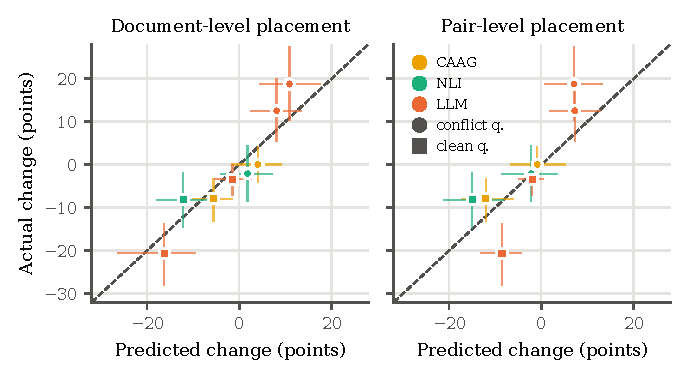
\includegraphics[width=\columnwidth]{generated/fig_placement.pdf}
\caption{Effect of real detectors predicted from the synthetic grid (x, with the 95\% bootstrap prediction interval)
against the measured effect (y, with its 95\% CI), for conflict ($\bullet$) and clean ($\blacksquare$) questions.
Left: detectors located by document-level behaviour; right: by pair precision, recall and direction precision.}
\label{fig:placement}
\end{figure}

\paragraph{The heuristic detector.}
CAAG, the detector we set out to study, scores a pair only if its MiniLM \citep{reimers2019sbert} cosine similarity reaches $\theta_s=0.65$. Its score
is the sum of a negation and contrast asymmetry term, a named-entity mismatch term (differing dates, numbers, money or
percentages) and a temporal-marker term, multiplied by the similarity; a pair is flagged at
$\theta_c=0.35$. Its per-pair flag rate on the confirmatory split ($6.22\%$) sets the random detector's rate.
As a neutral flag, CAAG did not beat random flags of the same volume, and
as a removal rule it only deleted correct passages (\dCaagRemClean\ points on clean questions, \dCaagRemConf\ on
conflict ones). Its false flags mostly hit pairs that should both be reported: 134 of 221 on the
hold-out are same-name ambiguity pairs, flagged by its entity-mismatch signal for differing dates or
numbers. We read this as a warning about lexical contradiction cues generally \citep{gururangan2018annotation},
not a particular threshold. Retuning shows why F1 misleads: over a 121-setting sweep, CAAG's
best pair F1 is \caagBestFOne, above NLI's, at $\theta_s=\caagBestThS$ and $\theta_c=\caagBestThC$, but it flags \caagBestRate\% of all pairs and \caagBestCleanFpr\% of clean questions, which our grid predicts
is harmful under removal (Appendix~\ref{app:grid}).

\paragraph{Original CAAG format.}
CAAG's flags in their original format, with typed lines and confidence scores (``factual conflict (confidence:
0.41)''), change accuracy by \origCaagAll\ points overall (\origCaagConf\ on conflict questions, \origCaagClean\ on
clean ones), no different from the uniform format.

\paragraph{Pilot study (exploratory).}
Before any confirmatory run, the 200-question pilot split, scored with the bidirectional metric, showed the same
pattern: oracle neutral flags changed conflict-question accuracy by $-$10.5 points, directional flags by
$+$11.8, and removing the suspect by $+$28.4. The pilots also showed that the original \textsc{remove} strategy,
which deletes an arbitrary side of each pair, removes correct documents, and led us to add directional formats,
synthetic direction precision and document-level placement. All pilot runs are released.

\paragraph{Phase-0 audit of CAAG on NarrativeQA.}
CAAG was designed for long-document QA. On 100 NarrativeQA \citep{kocisky2018narrativeqa} questions from 50 stories
(BM25 top-10 chunks from a single coherent story), it flags at least one pair in 54\% of questions, 166 pairs in all.
A single story rarely contradicts itself, so most flags are likely false. The flagged pairs are released for annotation.

\clearpage
\section{Further Results}
\label{app:more}

\begin{figure}[t]
\centering
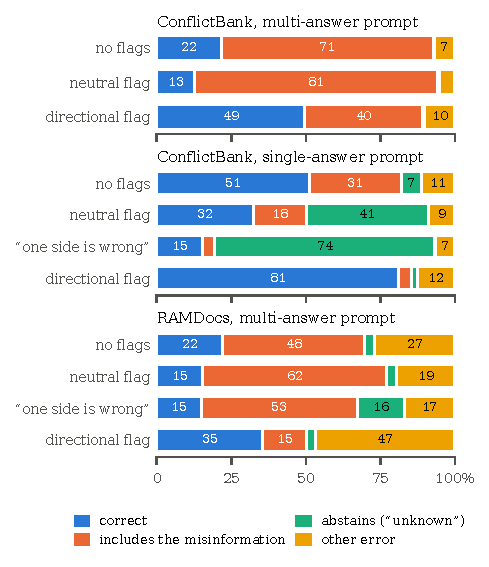
\includegraphics[width=\columnwidth]{generated/fig_answers.pdf}
\caption{What a flag does to answers on conflict questions (gpt-4o-mini, oracle pairs; share of answers, \%). The
answer policy decides how a neutral flag fails: told to give every valid answer, a model adds the misinformation;
told there is one answer, it abstains. Only the directional flag raises the share of correct answers. Categories are exclusive, correct (under the primary metric) taking precedence, so the misinformation share can be slightly lower than in Table~\ref{tab:risk}, which counts every answer containing a wrong answer under the bidirectional matcher.}
\label{fig:answers}
\end{figure}
\begin{table*}[t]
\centering\small
\setlength{\tabcolsep}{3.5pt}
\resizebox{\textwidth}{!}{%
\begin{tabular}{lrrrrrrrrrrrr}
\toprule
& \multicolumn{4}{c}{No flags} & \multicolumn{4}{c}{Oracle, neutral flag} & \multicolumn{4}{c}{Oracle, directional flag} \\
\cmidrule(lr){2-5}\cmidrule(lr){6-9}\cmidrule(lr){10-13}
Generator & Correct & Misinfo. & Abstain & Sel. & Correct & Misinfo. & Abstain & Sel. & Correct & Misinfo. & Abstain & Sel. \\
\midrule
\multicolumn{13}{l}{\emph{RAMDocs, multi-answer prompt}} \\
gpt-4o-mini & 22.1 & 47.7 & 3.4 & 22.8 & 15.3 & \textbf{61.9} & 5.0 & 16.2 & 35.5 & \textbf{14.9} & 2.9 & \textbf{36.5} \\
gpt-6-luna & 14.4 & 72.2 & 1.2 & 14.6 & 11.3 & 76.7 & 0.7 & 11.4 & 53.5 & \textbf{11.3} & 1.4 & \textbf{54.3} \\
Claude Haiku 5.5 & 25.2 & 55.2 & 2.2 & 25.7 & 26.4 & \textbf{47.2} & 2.2 & 27.0 & 53.5 & \textbf{6.7} & 2.9 & \textbf{55.1} \\
gpt-6.1-terra & 10.8 & 75.5 & 2.2 & 11.0 & 10.1 & 81.3 & 1.4 & 10.2 & 50.4 & \textbf{13.7} & 2.2 & \textbf{51.5} \\
Claude Sonnet 5.5 & 45.3 & 24.5 & 2.2 & 46.3 & 45.3 & 21.6 & 2.2 & 46.3 & 59.7 & \textbf{3.6} & 1.4 & \textbf{60.6} \\
\midrule
\multicolumn{13}{l}{\emph{ConflictBank, multi-answer prompt}} \\
gpt-4o-mini & 21.6 & 72.8 & 0.3 & 21.6 & 12.8 & \textbf{83.2} & 0.9 & \textbf{12.9} & 49.4 & \textbf{41.2} & 1.2 & \textbf{50.1} \\
gpt-4.1 & 13.0 & 82.7 & 0.7 & 13.1 & 6.7 & \textbf{90.7} & 0.3 & \textbf{6.7} & 36.0 & \textbf{58.3} & 1.0 & \textbf{36.4} \\
Qwen2.5-7B & 23.7 & 67.0 & 6.0 & 25.2 & 15.3 & \textbf{79.0} & 5.0 & \textbf{16.1} & 41.3 & \textbf{52.0} & 13.0 & \textbf{47.5} \\
\midrule
\multicolumn{13}{l}{\emph{ConflictBank, one-answer prompt}} \\
gpt-4o-mini & 51.1 & 31.0 & 6.7 & 54.8 & 32.4 & \textbf{17.7} & \textbf{41.0} & 55.0 & 81.2 & \textbf{4.2} & \textbf{2.1} & \textbf{83.0} \\
gpt-6-luna & 53.6 & 24.3 & 11.9 & 60.8 & 44.1 & \textbf{17.4} & \textbf{28.9} & 62.0 & 90.0 & \textbf{0.0} & \textbf{0.8} & \textbf{90.7} \\
Claude Haiku 5.5 & 66.8 & 22.0 & 1.2 & 67.6 & 67.4 & 22.1 & 0.9 & 68.0 & 90.1 & \textbf{0.2} & 1.1 & \textbf{91.1} \\
gpt-6.1-terra & 73.0 & 18.0 & 1.7 & 74.2 & 70.7 & 15.7 & 4.7 & 74.1 & 90.0 & \textbf{0.7} & 0.3 & \textbf{90.3} \\
Claude Sonnet 5.5 & 75.7 & 15.7 & 1.0 & 76.4 & 78.7 & 12.0 & 1.7 & 80.0 & 92.0 & 1.0 & 1.7 & 93.6 \\
gpt-4.1 & 64.7 & 27.3 & 1.7 & 65.8 & 56.7 & 21.7 & 14.0 & 65.9 & 91.3 & 0.3 & 1.7 & 92.9 \\
Qwen2.5-7B & 50.3 & 35.3 & 5.0 & 53.0 & 47.0 & 28.7 & 15.0 & 55.3 & 75.7 & 13.0 & 1.3 & 76.7 \\
\midrule
\multicolumn{13}{l}{\emph{ConflictBank, forced choice}} \\
gpt-4o-mini & 55.4 & 31.6 & 0.1 & 55.5 & 55.2 & 31.9 & 0.4 & 55.5 & 79.7 & \textbf{6.7} & 0.0 & \textbf{79.7} \\
gpt-6-luna & 64.6 & 25.8 & 0.0 & 64.6 & 66.1 & 22.0 & 0.0 & 66.1 & 91.0 & \textbf{0.1} & 0.0 & \textbf{91.0} \\
Claude Haiku 5.5 & 69.3 & 20.9 & 0.0 & 69.3 & 73.2 & \textbf{16.8} & 0.0 & \textbf{73.2} & 90.4 & \textbf{0.0} & 0.0 & \textbf{90.4} \\
gpt-6.1-terra & 77.7 & 14.7 & 0.0 & 77.7 & 77.3 & 13.3 & 0.0 & 77.3 & 92.3 & \textbf{0.3} & 0.0 & \textbf{92.3} \\
\bottomrule
\end{tabular}}
\caption{Risk and coverage on conflict questions (\%): strictly correct answers, answers that contain the
misinformation, abstentions (``unknown''), and selective accuracy (correct answers over non-abstained answers, pooled
over questions and seeds). \textbf{Bold}: the change from no flags is significant (H21 for
ConflictBank one-answer and forced; the paper's exploratory family elsewhere). The answer policy decides what a neutral
flag does: under a prompt that asks for every valid answer it adds the misinformation to the answer; under a one-answer
prompt that allows ``unknown'' it moves answers, misinformed and correct, into abstention; under forced choice it has
no abstention to trade.}
\label{tab:risk}
\end{table*}


\paragraph{Answer mix by prompt (Table~\ref{tab:risk}).} Table~\ref{tab:risk} gives the answer mix behind
\S\ref{sec:neutral}. Its correct and
selective-accuracy columns use the one-way matcher, and abstention needs no matcher. Its misinformation column counts
answers containing the misinformation under the bidirectional matcher, and the bold marks in that column rest on the
bidirectional value: from H21 in the ConflictBank one-answer and forced-choice panels, from the exploratory family
elsewhere. R12 (Appendix~\ref{app:rev11}) gives the one-way version, under which one bold mark is lost (\oneWayBoldLostCell). Table~\ref{tab:riskcov} and Figure~\ref{fig:riskcov} use the one-way matcher for every column.

\begin{table*}[t]
\centering\small
\setlength{\tabcolsep}{3.6pt}
\resizebox{\textwidth}{!}{%
\begin{tabular}{lrrrrrrrrrr}
\toprule
& \multicolumn{3}{c}{RAMDocs, gpt-4o-mini} & \multicolumn{2}{c}{RAMDocs, gpt-4.1} & \multicolumn{2}{c}{ConflictBank} & \multicolumn{2}{c}{CB majority} & \\
\cmidrule(lr){2-4}\cmidrule(lr){5-6}\cmidrule(lr){7-8}\cmidrule(lr){9-10}
Method & Lab. & Conflict & Clean & Lab. & Conflict & Conflict & Clean & Conflict & Clean & Calls \\
\midrule
No flags (plain), accuracy & 31.3 & 22.1 & 41.5 & 32.8$^\dagger$ & 19.4$^\dagger$ & 51.1 & 89.0 & 21.6 & 89.0 & 1 \\
\midrule
Instruction (v2) only & $+$2.3 & $+$5.3 & $-$1.1 & -- & $+$12.2 & -- & -- & -- & -- & 1 \\
Oracle, flag + instr. & $-$1.8 & $-$2.4 & $-$1.1 & $+$1.5$^\dagger$ & $+$5.8$^\dagger$ & -- & -- & -- & -- & 1 \\
Oracle, dir.\ flag + instr. & $+$6.4 & $+$13.2 & $-$1.1 & \textbf{$+$14.7}$^\dagger$ & \textbf{$+$30.9}$^\dagger$ & -- & -- & -- & -- & 1 \\
\midrule
MADAM-RAG & $+$5.7 & $+$3.6 & $+$7.9 & -- & -- & -- & -- & -- & -- & 9$\times$tok. \\
Astute RAG & \textbf{$-$15.6} & $-$8.4 & \textbf{$-$23.5} & -- & -- & $-$2.1 & $-$9.7 & $+$1.4 & $-$9.7 & 2 \\
Astute RAG (multi) & $-$5.9 & $-$1.2 & $-$11.1 & $+$2.3$^\dagger$ & $+$13.7$^\dagger$ & -- & -- & -- & -- & 2 \\
TrustRAG & \textbf{$-$17.5} & $-$11.3 & \textbf{$-$24.3} & -- & -- & $-$9.7 & $-$4.0 & $+$6.8 & $-$4.0 & 3 \\
TrustRAG (multi) & \textbf{$-$18.1} & $-$12.2 & \textbf{$-$24.6} & $-$10.9$^\dagger$ & 0.0$^\dagger$ & -- & -- & -- & -- & 3 \\
Single call (name suspects, then answer) & $+$6.2 & $+$12.0 & $-$0.3 & -- & -- & $+$7.6 & $-$1.0 & $+$6.8 & $-$1.0 & 1 \\
\midrule
LLM detector, flag + instr. & $-$2.0 & $-$2.2 & $-$1.9 & -- & -- & -- & -- & -- & -- & 1+1 \\
LLM detector, dir.\ flag + instr. & $-$3.5 & $+$8.4 & \textbf{$-$16.7} & -- & -- & -- & -- & -- & -- & 1+1 \\
LLM detector, dir.\ flag & $+$4.9 & $+$12.5 & $-$3.4 & $+$8.7$^\dagger$ & $+$14.4$^\dagger$ & $+$8.4 & $-$4.7 & \textbf{$+$5.7} & $-$4.7 & 1+1 \\
LLM detector, remove suspect & 0.0 & $+$18.7 & \textbf{$-$20.6} & -- & \textbf{$+$20.6} & $+$7.9 & $-$7.0 & $+$7.0 & $-$7.0 & 1+1 \\
\bottomrule
\end{tabular}}
\caption{Resolution instructions, published baselines and a single-call baseline. First row: accuracy (\%, one-way
strict) with no flags; other rows: paired difference from it in points. RAMDocs uses the multi-answer prompt (it has
same-name questions with several answers); ConflictBank and its majority variant (three wrong-side passages, one
correct) use the single-answer prompt and gpt-4o-mini. \emph{Lab.}: labelled RAMDocs questions. 3 seeds, except
$^\dagger$: gpt-4.1 seed 0 only, relative to the seed-0 no-flag accuracy in the first row (other gpt-4.1 cells are
relative to its 3-seed no-flag accuracy, Table~\ref{tab:gpt41}). \emph{instr.}: the v2 reliability instruction. \emph{(multi)}: the baseline's final
step asks for every valid answer. \emph{Single call}: one call that names suspect passages, then answers. Calls per
question; \emph{1+1}: one detector call and one generator call. \textbf{Bold}: significant under the paper's single
scheme.}
\label{tab:baselines}
\end{table*}

\begin{table*}[t]
\centering\footnotesize
\setlength{\tabcolsep}{3pt}
\begin{tabular}{llrrrrrrrrrrr}
\toprule
& & \multicolumn{2}{c}{Detector} & & & & \multicolumn{4}{c}{Accuracy with} & \multicolumn{2}{c}{Flag minus} \\
\cmidrule(lr){3-4}\cmidrule(lr){8-11}\cmidrule(lr){12-13}
Detector & Generator & Right & Wrong & Gen.\ acc. & Score & Gain & flag & verdict & hint & det.\ alone & hint & det.\ alone \\
\midrule
gpt-4o-mini & gpt-6.1-terra & 67.0 & 30.3 & 73.0 & $-$4.7 & \textbf{$-$11.7} & 61.3 & -- & 67.7 & 51.1 & $-$6.3 & \textbf{$+$10.2} \\
gpt-4o-mini & Claude Haiku & 67.0 & 30.3 & 66.8 & $+$1.9 & $-$4.1 & 62.7 & 61.7 & 64.1 & 51.1 & $-$1.4 & \textbf{$+$11.6} \\
gpt-6.1-terra & gpt-6.1-terra & 29.7 & 4.3 & 73.0 & $+$2.7 & $+$2.7 & 75.7 & -- & 66.0 & 73.0 & \textbf{$+$9.7} & $+$2.7 \\
gpt-4o-mini & gpt-4.1 & 67.0 & 30.3 & 64.7 & $+$4.0 & $-$2.3 & 62.3 & -- & 61.7 & 51.1 & $+$0.7 & \textbf{$+$11.2} \\
gpt-6.1-terra & Claude Haiku & 29.7 & 4.3 & 66.8 & $+$4.3 & \textbf{$+$4.1} & 70.9 & 68.2 & 59.9 & 73.0 & \textbf{$+$11.0} & $-$2.1 \\
gpt-6.1-terra & gpt-4.1 & 29.7 & 4.3 & 64.7 & $+$4.7 & \textbf{$+$5.0} & 69.7 & -- & 68.0 & 73.0 & $+$1.7 & $-$3.3 \\
gpt-6-luna & gpt-6.1-terra & 45.7 & 6.7 & 73.0 & $+$5.3 & $+$2.7 & 75.7 & -- & 66.0 & 53.6 & \textbf{$+$9.7} & \textbf{$+$22.1} \\
gpt-6-luna & Claude Haiku & 45.7 & 6.7 & 66.8 & $+$7.1 & \textbf{$+$5.0} & 71.8 & 69.7 & 61.4 & 53.6 & \textbf{$+$10.3} & \textbf{$+$18.2} \\
gpt-6.1-terra & gpt-6-luna & 29.7 & 4.3 & 53.6 & $+$7.7 & \textbf{$+$7.3} & 60.9 & 60.6 & 66.7 & 73.0 & $-$5.8 & \textbf{$-$12.1} \\
gpt-6-luna & gpt-4.1 & 45.7 & 6.7 & 64.7 & $+$7.7 & \textbf{$+$6.3} & 71.0 & -- & 61.3 & 53.6 & \textbf{$+$9.7} & \textbf{$+$17.4} \\
Claude Haiku & Claude Haiku & 61.7 & 11.3 & 66.8 & $+$9.8 & \textbf{$+$5.7} & 72.4 & 71.6 & 61.3 & 66.8 & \textbf{$+$11.1} & \textbf{$+$5.7} \\
Claude Sonnet & Claude Haiku & 65.0 & 9.7 & 66.8 & $+$11.7 & \textbf{$+$8.2} & 75.0 & 73.8 & 60.4 & 75.7 & \textbf{$+$14.6} & $-$0.7 \\
gpt-6.1-terra & Qwen2.5-7B & 31.0 & 4.0 & 50.3 & $+$11.7 & \textbf{$+$8.0} & 58.3 & 55.0 & 62.3 & 73.0 & $-$4.0 & \textbf{$-$14.7} \\
gpt-6.1-terra & gpt-4o-mini & 31.3 & 4.0 & 51.1 & $+$12.8 & \textbf{$+$9.6} & 60.7 & 58.4 & 60.6 & 73.0 & $+$0.1 & \textbf{$-$12.3} \\
gpt-6-luna & gpt-6-luna & 45.7 & 6.7 & 53.6 & $+$13.8 & \textbf{$+$11.1} & 64.7 & 65.3 & 56.4 & 53.6 & \textbf{$+$8.2} & \textbf{$+$11.1} \\
gpt-4o-mini & gpt-6-luna & 67.0 & 30.3 & 53.6 & $+$14.7 & \textbf{$+$8.6} & 62.1 & 61.9 & 56.1 & 51.1 & $+$6.0 & \textbf{$+$11.0} \\
gpt-4.1 & gpt-6.1-terra & 79.0 & 8.0 & 73.0 & $+$15.7 & \textbf{$+$7.3} & 80.3 & -- & 69.7 & 64.7 & \textbf{$+$10.7} & \textbf{$+$15.7} \\
gpt-4o-mini & Qwen2.5-7B & 67.0 & 30.3 & 50.3 & $+$17.3 & \textbf{$+$7.3} & 57.7 & 54.7 & 53.3 & 51.1 & $+$4.3 & $+$6.6 \\
gpt-4o-mini & gpt-4o-mini & 67.0 & 30.3 & 51.1 & $+$17.6 & \textbf{$+$8.4} & 59.6 & 57.1 & 52.4 & 51.1 & $+$7.1 & \textbf{$+$8.4} \\
gpt-6-luna & gpt-4o-mini & 45.7 & 6.7 & 51.1 & $+$19.1 & \textbf{$+$13.7} & 64.8 & 63.3 & 56.7 & 53.6 & \textbf{$+$8.1} & \textbf{$+$11.2} \\
Claude Haiku & gpt-6-luna & 61.7 & 11.3 & 53.6 & $+$19.1 & \textbf{$+$14.3} & 67.9 & 68.7 & 63.0 & 66.8 & $+$4.9 & $+$1.1 \\
gpt-6-luna & Qwen2.5-7B & 48.0 & 6.7 & 50.3 & $+$19.7 & \textbf{$+$12.0} & 62.3 & 59.7 & 58.0 & 53.6 & $+$4.3 & \textbf{$+$8.8} \\
gpt-4.1 & Claude Haiku & 79.0 & 8.0 & 66.8 & $+$20.2 & \textbf{$+$11.0} & 77.8 & 76.0 & 63.7 & 64.7 & \textbf{$+$14.1} & \textbf{$+$13.1} \\
gpt-4.1 & gpt-4.1 & 79.0 & 8.0 & 64.7 & $+$20.7 & \textbf{$+$11.7} & 76.3 & -- & 63.3 & 64.7 & \textbf{$+$13.0} & \textbf{$+$11.7} \\
Claude Haiku & gpt-4o-mini & 61.7 & 11.3 & 51.1 & $+$21.3 & \textbf{$+$13.0} & 64.1 & 62.7 & 57.9 & 66.8 & $+$6.2 & $-$2.7 \\
Claude Sonnet & gpt-6-luna & 65.0 & 9.7 & 53.6 & $+$22.8 & \textbf{$+$18.1} & 71.7 & 72.9 & 67.8 & 75.7 & $+$3.9 & $-$4.0 \\
Claude Sonnet & gpt-4o-mini & 65.0 & 9.7 & 51.1 & $+$28.1 & \textbf{$+$15.9} & 67.0 & 69.0 & 61.2 & 75.7 & $+$5.8 & \textbf{$-$8.7} \\
gpt-4.1 & gpt-6-luna & 79.0 & 8.0 & 53.6 & $+$30.1 & \textbf{$+$21.3} & 74.9 & 76.8 & 61.2 & 64.7 & \textbf{$+$13.7} & \textbf{$+$10.2} \\
gpt-4.1 & gpt-4o-mini & 79.0 & 8.0 & 51.1 & $+$33.8 & \textbf{$+$18.6} & 69.7 & 67.6 & 57.9 & 64.7 & \textbf{$+$11.8} & $+$5.0 \\
gpt-4.1 & Qwen2.5-7B & 79.3 & 7.7 & 50.3 & $+$36.7 & \textbf{$+$16.0} & 66.3 & 63.3 & 57.7 & 64.7 & $+$8.7 & $+$1.7 \\
\bottomrule
\end{tabular}
\caption{Every detector--generator cell of H24 and H27 (ConflictBank, one-answer prompt, 300 conflict questions; \%),
sorted by the exploratory score. \emph{Right}: the detector's hit rate, the share of questions on which it flags the true
contradiction and names exactly its misinformation passage (computed on the detections that cell's generator saw;
its direction precision with `both' and `unclear' verdicts counted as misses, unlike Table~\ref{tab:terms}, i.e.\ the
same share among questions where it flags the true pair, pooled over its cells, is
gpt-4o-mini \dirPrecMini\%, gpt-4.1 \dirPrecFour\%, gpt-6-luna \dirPrecLuna\%, gpt-6.1-terra \dirPrecTerra\%, Claude Haiku
\dirPrecHaiku\% and Claude Sonnet \dirPrecSonnet\%); \emph{Wrong}: share on which it marks a correct passage as suspect;
\emph{Gen.\ acc.}: the generator's accuracy with no flags; \emph{Score}: the mean over the 300 questions of [right direction and the generator errs] minus [a
correct passage marked and the generator is right]; \emph{Gain}: the LLM directional flag's change in points. \emph{Verdict}: the detector's judgement passed as an answer key (``the answer $X$ is false'' for the answer its suspect passage supports; H30). \emph{Hint}: the
generator given the detector model's own plain answer, with no passage marked (H27); \emph{det.\ alone}: the detector
model's own plain accuracy. A detector's statistics can differ slightly between generators because concurrent runs
made independent detector calls (up to \detDiffMax\ of 400 questions differ for one detector). Bold: significant under
the paper's scheme (Gain: exploratory family; hint and det.\ alone columns: H27, Holm across cells).}
\label{tab:cells}
\end{table*}

\begin{table}[t]
\centering\footnotesize
\setlength{\tabcolsep}{3pt}
\resizebox{\columnwidth}{!}{%
\begin{tabular}{lr}
\toprule
\multicolumn{2}{l}{\emph{Cell level (30 cells): accuracy with the flag, $A$}} \\
$A \sim D + G$: coefficient of $D$ (hit rate) & 0.09 [0.03, 0.16] \\
\quad coefficient of $G$ & 0.46 [0.36, 0.55] \\
$A \sim D$ + generator FE, permutation of $D$ & $p=0.29$ \\
$A \sim P + R$ + gen.\ FE: precision $P$ & \recPCoef\ \recPCoefCI; $p=\recPPerm$ \\
\quad recall $R$ & \recRCoef\ \recRCoefCI; $p=\recRPerm$ \\
\midrule
\multicolumn{2}{l}{\emph{Leave one detector out: $R^2$ for the gain}} \\
$G$ only & 0.17 \\
gap $D-G$ (registered) & $-$0.21 \\
$P+R+G$ & \recCvPRG \\
score (exploratory) & 0.62 \\
\midrule
\multicolumn{2}{l}{\emph{Question level, question/detector/generator FE (points)}} \\
detector right on $q$ & \qfeD\ \qfeDCI \\
detector marks a correct passage & \qfeW\ \qfeWCI \\
\bottomrule
\end{tabular}}

\vspace{4pt}
\resizebox{\columnwidth}{!}{%
\begin{tabular}{lrrrrr}
\toprule
& \multicolumn{3}{c}{H24 cells (observational)} & \multicolumn{2}{c}{H31 (randomised)} \\
\cmidrule(lr){2-4}\cmidrule(lr){5-6}
Generator & right & wrong & wrong, abst. & right & wrong \\
\midrule
Qwen2.5-7B & 61 & 68 & 6 & -- & -- \\
Claude Haiku & 57 & 59 & 18 & 63 & 64 \\
gpt-4.1 & 69 & 65 & 13 & -- & -- \\
gpt-4o-mini & 66 & 52 & 24 & 57 & 51 \\
gpt-6-luna & 75 & 57 & 16 & 72 & 77 \\
gpt-6.1-terra & 68 & 75 & 4 & 67 & 95 \\
\bottomrule
\end{tabular}}
\caption{H24 re-analysed (PR\S15.4, PR\S16.4; data already seen). $D$: hit rate (the detector flags the gold pair and names
exactly its misinformation passage); $P$: direction precision (of those gold-pair flags, the share naming it); $R$: recall (the
share of questions whose gold pair is flagged); $G$: the generator's no-flag accuracy. CIs: 2,000 question resamples
shared across cells (300 with question fixed effects; the leave-one-detector-out range of the question-level
coefficients is \qfeDLodo\ and \qfeWLodo). $p$: exact permutation of the detectors' values across the six detectors; the design is unbalanced (the Claude
detectors serve three generators), so detectors are only approximately exchangeable.
Lower table, one definition of following: a right flag is followed when the flagged answer is correct (questions the
generator gets wrong in every plain seed); a wrong flag is followed when the flagged answer contains the
misinformation (questions it gets right in every plain seed); \emph{abst.}: the flagged answer abstains instead. With
no flag, a held-out plain seed changes outcome on at most \folNullMax\% of such questions.}
\label{tab:h24redo}
\end{table}

\begin{table*}[t]
\centering\footnotesize
\setlength{\tabcolsep}{4pt}
\begin{tabular}{llrllr}
\toprule
Policy & Setting & Neutral flag & Policy & Setting & Neutral flag \\
\midrule
forced & CB forced, gpt-6.1-terra & $-$0.3 & multi & RAMDocs, Claude Haiku & $+$1.2 \\
forced & CB forced, gpt-4o-mini & $-$0.2 & one & CB one-answer, gpt-4o-mini & $-$18.7 \\
forced & CB forced, gpt-6-luna & $+$1.6 & one & CB one-answer, gpt-6-luna & $-$9.4 \\
forced & CB forced, Claude Haiku & $+$3.9 & one & CB one-answer, gpt-4.1 & $-$8.0 \\
minimal & CB minimal, gpt-4o-mini & $-$18.1 & one & CB majority, gpt-6.1-terra & $-$3.7 \\
minimal & RAMDocs, gpt-4.1 (minimal) & $-$11.0 & one & CB one-answer, Qwen2.5-7B & $-$3.3 \\
minimal & RAMDocs, Qwen2.5-7B (minimal) & $-$5.8 & one & CB one-answer, gpt-6.1-terra & $-$2.3 \\
minimal & RAMDocs, gpt-4o-mini (minimal) & $-$5.3 & one & RAGuard, gpt-6-luna & 0.0 \\
multi & CB multi-answer, gpt-4o-mini & $-$8.8 & one & RAGuard, Claude Haiku & $+$0.3 \\
multi & RAMDocs, gpt-4.1 (multi-answer) & $-$8.6 & one & CB one-answer, Claude Haiku & $+$0.7 \\
multi & CB multi-answer, Qwen2.5-7B & $-$8.3 & one & CB majority, gpt-4o-mini & $+$1.1 \\
multi & RAMDocs, gpt-4o-mini (multi-answer) & $-$6.7 & one & RAGuard, gpt-6.1-terra & $+$2.4 \\
multi & CB multi-answer, gpt-4.1 & $-$6.3 & one & CB one-answer, Claude Sonnet & $+$3.0 \\
multi & RAMDocs, Qwen2.5-7B (multi-answer) & $-$5.8 & one & RAGuard, gpt-4o-mini & $+$3.2 \\
multi & RAMDocs, gpt-6-luna & $-$3.1 & one & CB majority, Claude Haiku & $+$4.3 \\
multi & RAMDocs, gpt-6.1-terra & $-$0.7 & one & RAGuard, Claude Sonnet & $+$4.4 \\
multi & RAMDocs, Claude Sonnet & 0.0 & one & CB majority, gpt-6-luna & $+$6.6 \\
\midrule
\multicolumn{6}{l}{\emph{Multilevel model (random effects for generator, benchmark and setting; REML)}} \\
\multicolumn{3}{l}{pooled, all settings} & \multicolumn{3}{l}{\neuMlMu\ \neuMlCI; prediction interval \neuMlPI} \\
\multicolumn{3}{l}{pooled, multi-answer prompt (10 settings)} & \multicolumn{3}{l}{$-$3.5 [$-$6.4, $-$0.6]} \\
\multicolumn{3}{l}{pooled, minimal prompt (4 settings)} & \multicolumn{3}{l}{$-$12.1 [$-$23.2, $-$1.0]} \\
\multicolumn{3}{l}{pooled, one answer prompt (16 settings)} & \multicolumn{3}{l}{$-$0.4 [$-$5.3, $+$4.5]} \\
\multicolumn{3}{l}{pooled, forced prompt (4 settings)} & \multicolumn{3}{l}{$+$1.5 [$-$1.7, $+$4.8]} \\
\midrule
\multicolumn{6}{l}{\emph{Meta-regression (same model)}} \\
\multicolumn{3}{l}{intercept (OpenAI, one answer, generated)} & \multicolumn{3}{l}{$-$2.1 [$-$7.3, $+$3.0]} \\
\multicolumn{3}{l}{several answers allowed} & \multicolumn{3}{l}{$-$3.7 [$-$8.2, $+$0.8]} \\
\multicolumn{3}{l}{forced (no unknown)} & \multicolumn{3}{l}{$+$6.0 [$+$1.7, $+$10.3]} \\
\multicolumn{3}{l}{Anthropic} & \multicolumn{3}{l}{$+$4.6 [$+$1.5, $+$7.7]} \\
\multicolumn{3}{l}{Qwen} & \multicolumn{3}{l}{$+$0.6 [$-$3.9, $+$5.1]} \\
\multicolumn{3}{l}{natural misinformation (RAGuard)} & \multicolumn{3}{l}{$+$2.2 [$-$7.2, $+$11.6]} \\
\bottomrule
\end{tabular}
\caption{The 34 settings on misinformation benchmarks (RAMDocs, ConflictBank and its one-answer, minimal,
forced-choice and majority variants, RAGuard) in which the oracle neutral flag was run; WikiContradict (genuine
conflicts) and CONFLICTS are not pooled (conflict questions, change in
points), grouped by answer policy. The pooled estimate was registered as exploratory (PR\S13.4) and the multilevel model,
the policy split and the moderators in PR\S16.4; they use data already seen. The prediction interval describes this
design space (our generators, benchmarks and prompts), not deployments in general. \emph{Natural misinformation} is
RAGuard only; RAMDocs' misinformation is synthetic. The moderator \emph{several answers allowed} codes the
multi-answer and minimal prompts together, against one-answer prompts; the policy rows above separate them. Settings
share questions, so the model is fitted with their sampling covariance, estimated by a joint question bootstrap
(PR\S17.1: each replicate resamples each benchmark's questions once for every setting that uses them). Treating the
settings as independent gives [$-$5.5, $+$2.2]; conditional on these settings (question sampling only) the pooled
effect is \neuMlCIDesign.}
\label{tab:pooled}
\end{table*}

\begin{table*}[t]
\centering\footnotesize
\setlength{\tabcolsep}{3.5pt}
\resizebox{\textwidth}{!}{%
\begin{tabular}{lrrrrrrrrr}
\toprule
& \multicolumn{4}{c}{Neutral flag, utility change at misinformation cost $c$} & Dir.\ flag & \multicolumn{4}{c}{Neutral flag: plain answer $\to$ flagged answer (null)} \\
\cmidrule(lr){2-5}\cmidrule(lr){6-6}\cmidrule(lr){7-10}
Setting & $c=0$ & $c=1$ & $c=2$ & $c=4$ & $c=2$ & mis.$\to$abst. & mis.$\to$corr. & corr.$\to$abst. & corr.$\to$mis. \\
\midrule
RAMDocs, gpt-4o-mini (multi-answer) & \textbf{$-$6.7} & \textbf{$-$20.9} & \textbf{$-$35.0} & \textbf{$-$63.3} & \textbf{$+$79.1} & 1 (0) & 2 (2) & 0 (0) & 29 (3) \\
RAMDocs, gpt-6-luna & \textbf{$-$3.1} & $-$7.7 & $-$12.2 & $-$21.3 & \textbf{$+$160.9} & 0 (0) & 1 (3) & 0 (0) & 22 (16) \\
RAMDocs, Claude Haiku & $+$1.2 & $+$9.1 & \textbf{$+$17.0} & \textbf{$+$32.9} & \textbf{$+$125.2} & 0 (0) & 9 (4) & 0 (0) & 5 (9) \\
CB multi-answer, gpt-4o-mini & \textbf{$-$8.8} & \textbf{$-$19.2} & \textbf{$-$29.7} & \textbf{$-$50.6} & \textbf{$+$91.0} & 0 (0) & 4 (3) & 1 (0) & 55 (9) \\
CB one-answer, gpt-4o-mini & \textbf{$-$18.7} & $-$5.3 & $+$8.0 & \textbf{$+$34.7} & \textbf{$+$83.7} & 45 (2) & 7 (3) & 37 (1) & 5 (2) \\
CB one-answer, gpt-6-luna & \textbf{$-$9.4} & $-$2.6 & $+$4.3 & $+$18.1 & \textbf{$+$85.1} & 27 (10) & 12 (13) & 20 (6) & 5 (6) \\
CB one-answer, gpt-6.1-terra & $-$2.3 & 0.0 & $+$2.3 & $+$7.0 & \textbf{$+$51.7} & 2 (--) & 26 (--) & 4 (--) & 5 (--) \\
CB one-answer, Claude Haiku & $+$0.7 & $+$0.6 & $+$0.4 & $+$0.2 & \textbf{$+$66.9} & 0 (0) & 25 (16) & 0 (0) & 8 (5) \\
CB one-answer, Claude Sonnet & $+$3.0 & $+$6.7 & $+$10.3 & $+$17.7 & \textbf{$+$45.7} & 2 (--) & 34 (--) & 0 (--) & 3 (--) \\
CB forced, gpt-4o-mini & $-$0.2 & $-$0.6 & $-$0.9 & $-$1.6 & \textbf{$+$74.0} & 1 (0) & 19 (4) & 0 (0) & 11 (2) \\
CB majority, gpt-4o-mini & $+$1.1 & \textbf{$+$24.6} & \textbf{$+$48.0} & \textbf{$+$94.9} & \textbf{$+$118.2} & 26 (1) & 11 (2) & 22 (1) & 8 (5) \\
RAGuard, gpt-4o-mini & $+$3.2 & $+$6.6 & $+$10.0 & $+$16.8 & \textbf{$+$34.6} & 12 (3) & 7 (3) & 8 (6) & 4 (2) \\
RAGuard, gpt-6-luna & 0.0 & $-$1.1 & $-$2.3 & $-$4.5 & \textbf{$+$29.3} & 10 (9) & 6 (9) & 8 (9) & 7 (8) \\
RAGuard, Claude Haiku & $+$0.3 & $-$1.8 & $-$4.0 & $-$8.3 & \textbf{$+$26.5} & 7 (6) & 4 (4) & 11 (9) & 6 (3) \\
\bottomrule
\end{tabular}}
\caption{Abstention-aware view of the oracle flags (conflict questions; PR\S15.4 and PR\S16.4, re-analyses of data already
seen). Utility per answer: $+1$ correct, $-c$ if it contains the misinformation, 0 for abstaining or any other wrong
answer; $c=0$ is strict accuracy. Bold: significant in one Holm family per $c$ over all \nUtilSixSettings\ settings of
Table~\ref{tab:pooled} (a selection is shown). Right: of the question--seed pairs whose plain answer contained the
misinformation (or was correct), the share whose flagged answer abstained, was correct or contained the misinformation;
in brackets the same share between two plain runs with different seeds, the churn with no flag.}
\label{tab:utility}
\end{table*}


\paragraph{H24 is supported only mechanically.} The registered H24 tests relate a crossed cell's gain to the gap
between the detector's and the generator's reliability. The generator's no-flag accuracy enters both sides of both
tests (\prs{13.3}), so the correlation is expected whatever the detector does. We record H24's status as
\emph{supported (mechanical)}; the ``supported'' in the hypothesis tables should be read that way. Five of the
\hTwentyFourCells\ cells existed when H24 was registered. Table~\ref{tab:h24redo} re-analyses the cells within
generators (exploratory).

\paragraph{Pooled summaries describe these 34 settings only (Table~\ref{tab:pooled}).} The body reports no pooled
estimate. Table~\ref{tab:pooled} keeps the summaries that \prs{13.4}, \prs{16.4} and \prs{17.1.1} registered, each
after the per-setting effects were seen. They describe these \neuMlK\ settings, which over-represent ConflictBank
prompt variants sharing one question pool. They are not estimates for any wider set of generators, benchmarks or
prompts, and no claim rests on them. The multilevel mean is \neuMlMu\ \neuMlCI\ (prediction interval \neuMlPI;
\neuMlCIDesign\ conditional on these settings), and the equal-weight mean of \prs{17.1.1} is \neuMlEqual\
\neuMlEqualCI. The moderators were coded after the per-setting effects were known (\prs{16.4.1}). With seven
generators and four benchmarks the variance components are poorly identified, and the RAGuard and Qwen moderators each
coincide with one level of a random effect.

\subsection{Where the directional flag fails (exploratory)}
\label{app:single}
After seeing the minimal-skeleton run, we split conflict questions by gold-answer count. \nConfMulti\ of
\the\numexpr\nConfMulti+\nConfSingle\relax\ have several (same-name ambiguity \emph{and} misinformation), and a strict
answer must list all. On the \nConfSingle\ single-answer conflict questions, the directional flag's estimate
is positive in every setting, from \yQwenSingleOracleDir\ points (Qwen) to \yMiniSingleOracleDir\ (gpt-4o-mini), both
with the default skeleton. On multi-answer questions it changes little except with gpt-4.1 (gpt-4o-mini
\yMiniMultiOracleDir, and \yMiniMinMultiOracleDir\ with the minimal skeleton; gpt-4.1 \yFourMultiOracleDir). One untested
reading: a warning about one passage makes the smaller models more conservative about legitimate
alternatives too. Removal, which needs no warning to be acted on, gains in both groups.

\subsection{Real detectors}
CAAG flags \cleanFprCaag\% of clean questions. Its neutral flags do not beat random flags at the same rate (H5;
\dCaagFlagAll\ vs.\ \dRandFlagAll\ points overall). The 90\% CI of the difference, [\tostLo, \tostHi], rules out a
gain above \tostHi\ points but does not establish equivalence within $\pm$\tostMargin\ points (TOST). The
addendum registered the LLM detector's directional-versus-neutral comparison as exploratory.
Under the bidirectional metric, the LLM detector's directional flag costs clean questions \arLlmDirClean\ points. With
gpt-4.1 generating, its gain over all 300 questions (\gptLlmDirAll) is significant after Holm, but the 35
unlabelled questions contribute disproportionately, gaining \agptexclLlmDir\ points. On labelled
questions it is \gptlabLlmDir\ \gptlabLlmDirCI. On ConflictBank the NLI cross-encoder flags no pair under the
registered window: the benchmark's passages are long, LLM-written and agree on all but the one fact, and the truncated
pair rarely contains it.

\paragraph{The single call on clean questions.} Asked in one call to name suspect passages and then answer, gpt-6-luna,
gpt-6.1-terra and Claude Haiku name passages as suspect even on clean questions and often abstain. On ConflictBank's
clean questions the single call changes their accuracy by \zSgLunaSelfIdentifyClean\ points
\zSgLunaSelfIdentifyCleanCI\ (gpt-6-luna), \zSgTerraSelfIdentifyClean\ \zSgTerraSelfIdentifyCleanCI\ (gpt-6.1-terra)
and \zSgHaikuSelfIdentifyClean\ \zSgHaikuSelfIdentifyCleanCI\ (Claude Haiku). Table~\ref{tab:cb} gives the single
call's effects on conflict questions; no table carries these clean-question losses. Used as two-call detectors on
ConflictBank-fresh, the same three models flag no clean question, so their clean-question rows in
Table~\ref{tab:fresh} are zero. The loss therefore belongs to the single-call format. We ran these models in a single
call only on ConflictBank, so whether they treat generated passages differently from real ones is untested.

\paragraph{Reasoning models on RAMDocs.} Without flags, gpt-6-luna and gpt-6.1-terra are
strictly correct on few RAMDocs conflict questions because the default prompt asks for every valid answer. They give
\mixRdLunaNAnswers\ and \mixRdTerraNAnswers\ answers on average and recover \mixRdLunaRecall\% and
\mixRdTerraRecall\% of gold answers, but \mixRdLunaMisinfo\% and \mixRdTerraMisinfo\% of their answers include
the misinformation.

\paragraph{Detector parsing.} The LLM detectors' JSON failed to parse on \parseFailTotal\ of \parseFailN\ ConflictBank
questions (a Claude Sonnet output), counted as flagging nothing.

\subsection{A second detector model on RAMDocs}
Replacing the gpt-4o-mini detector with Qwen2.5-7B (gpt-4o-mini still generates) gives a much less selective
detector, flagging \qdetFpr\% of clean RAMDocs questions, with direction precision \qdetDir\% (as defined in
Table~\ref{tab:detectors}). Its directional flag changes accuracy by \zQDetLlmDirFlagDirectionalConflict\ points on
conflict questions and \zQDetLlmDirFlagDirectionalClean\ on clean ones; its neutral flag, by
\zQDetLlmDirFlagConflict. Removal again trades a conflict-question gain (\zQDetLlmDirRemoveSuspectConflict) for a
clean-question loss (\zQDetLlmDirRemoveSuspectClean). With this one detector on one benchmark, the pattern matches the
gpt-4o-mini detector's; it cannot show whether the conclusions depend on the detector's model family.

\subsection{CONFLICTS}
On the 237 CONFLICTS questions with a reference answer (exploratory, 3 seeds), no condition moves accuracy
significantly (Table~\ref{tab:conflicts}). Only 69 of them have a conflict, most of these from outdated information
and few from misinformation, and the benchmark has no passage labels or oracle pairs. It is underpowered for our
question and can neither confirm nor refute our findings.

\clearpage
\section{Semantic Re-score, Label Audits and Selection}
\label{app:semantic}
\begin{table*}[t]
\centering\scriptsize
\setlength{\tabcolsep}{4pt}
\begin{tabular}{llrrr}
\toprule
Setting & Contrast & Matcher (points) & Judge (points) & Judge $-$ matcher \\
\midrule
RAMDocs, gpt-4o-mini & neutral flag vs plain & $-$4.2 [$-$9.2, 0.0] & $-$2.5 [$-$9.2, $+$4.2] & $+$1.7 [$-$3.3, $+$6.7] \\
ConflictBank, gpt-4o-mini & neutral flag vs plain & $-$20.0 [$-$27.5, $-$12.5] & $-$21.7 [$-$29.2, $-$14.2] & $-$1.7 [$-$4.2, 0.0] \\
ConflictBank, Claude Haiku & neutral flag vs plain & $+$3.3 [$-$3.3, $+$10.0] & $+$6.7 [$+$0.8, $+$13.3] & $+$3.3 [0.0, $+$7.5] \\
RAMDocs, gpt-4o-mini & oracle directional flag vs answer key & $-$0.8 [$-$5.8, $+$4.2] & $+$0.8 [$-$8.3, $+$10.0] & $+$1.7 [$-$6.7, $+$10.0] \\
ConflictBank, gpt-4o-mini & oracle directional flag vs answer key & $+$10.8 [$+$4.2, $+$17.5] & $+$12.5 [$+$6.7, $+$19.2] & $+$1.7 [$-$1.7, $+$5.0] \\
ConflictBank, gpt-6-luna & oracle directional flag vs answer key & $-$1.7 [$-$5.8, $+$2.5] & 0.0 [$-$3.3, $+$3.3] & $+$1.7 [$-$1.7, $+$5.0] \\
ConflictBank, gpt-4o-mini & LLM directional flag vs verdict key & $+$3.3 [$-$2.5, $+$9.2] & $+$6.7 [$+$0.8, $+$12.5] & $+$3.3 [0.0, $+$7.5] \\
ConflictBank, gpt-6-luna & LLM directional flag vs verdict key & $-$0.8 [$-$3.3, $+$1.7] & 0.0 [$-$2.5, $+$2.5] & $+$0.8 [$-$1.7, $+$4.2] \\
ConflictBank, gpt-4o-mini & randomised directional flag vs plain & $+$4.2 [$-$5.8, $+$15.0] & $+$6.7 [$-$3.3, $+$16.7] & $+$2.5 [0.0, $+$5.8] \\
ConflictBank, Claude Haiku & randomised directional flag vs plain & $-$7.5 [$-$18.3, $+$3.3] & $-$6.7 [$-$17.5, $+$4.2] & $+$0.8 [$-$1.7, $+$3.3] \\
\bottomrule
\end{tabular}

\vspace{4pt}
\begin{tabular}{lrrrrr}
\toprule
Condition & Outputs & Matcher (\%) & Judge (\%) & Judge only (\%) & Matcher only (\%) \\
\midrule
answer key & 360 & 67.8 & 77.8 & 10.3 & 0.3 \\
directional flag (LLM) & 240 & 59.6 & 62.5 & 3.8 & 0.8 \\
directional flag (oracle) & 360 & 70.6 & 82.2 & 11.7 & 0.0 \\
neutral flag (oracle) & 360 & 36.9 & 43.3 & 6.9 & 0.6 \\
no flag & 600 & 48.8 & 53.3 & 5.2 & 0.7 \\
randomised direction (H31) & 240 & 54.6 & 59.6 & 5.0 & 0.0 \\
verdict key (LLM) & 240 & 58.3 & 59.2 & 2.1 & 1.2 \\
\bottomrule
\end{tabular}
\caption{Semantic re-score (PR\S17.3; exploratory). An outside-family judge (gemini-3.5-flash-lite, temperature 0) reads
the question, the reference and known wrong answers and the response, and classifies the final answer; judge-strict
means it gives the reference answer, asserts no wrong one and does not abstain. Top: each contrast on the same
120 conflict questions (seed 0) under the matcher and the judge, and their difference, with question-bootstrap
95\% CIs. Bottom: per condition, the share scored correct by each and the shares where only one does. The judge is
an LLM given the answer keys: it checks the matcher's semantics, not the benchmark labels.}
\label{tab:semantic}
\end{table*}

\paragraph{An outside-family judge leaves the directional conclusions intact (\prs{17.3}).} To
check whether the matcher's errors differ by condition, an outside-family LLM re-scored both
arms of \semK\ contrasts on the same \semNq\ conflict questions each (gemini-3.5-flash-lite; Table~\ref{tab:semantic}).
\prs{17.3} named Gemini 2.5 Flash, closed to new users. Given the gold and wrong answers, the judge tests the
scorer, not the benchmark labels. Judge and matcher agree on \semAgree\% of \semN\ outputs. Almost all
disagreements are answers the judge accepts and the matcher rejects (aliases, paraphrases, partial forms).
Their share depends on condition: \semJudgeOnlyKey\% of answer-key outputs and \semJudgeOnlyDir\% of oracle-directional ones,
against \semJudgeOnlyPlain\% without a flag. The failure of most concern, a final answer such as
``$Y$, not $X$'' counted as asserting the wrong answer $X$, occurs in \semRejected\% of outputs. Since
both arms gain, the judge moves every contrast by \semDidMin\ to \semDidMax\ points. One small contrast changes sign (RAMDocs oracle flag against answer key, \semTwentyThreeRDMiniM\ to \semTwentyThreeRDMiniJ).
Two whose matcher intervals include zero exclude it under the judge (unadjusted): Claude Haiku's neutral flag
(\semNeuCBsHaikuJ) and gpt-4o-mini's LLM flag against its verdict key (\semThirtyCBsMiniM\ to \semThirtyCBsMiniJ, outside $\pm$3). With \semNq\ questions per contrast the re-score's
intervals are too wide to test the $\pm$3-point equivalence claims; re-scored in full, neither holds
(Appendix~\ref{app:fresh}).

\paragraph{A within-family judge check.} Before the outside-family re-score, gpt-6.1-terra judged \judgeN\
stratified conflict-question outputs and agreed with the primary metric on \judgeAgree\% ($\kappa=\judgeKappa$).
gpt-6.1-terra is itself one of the generators whose outputs it judged, so this check is within-family. The
outside-family re-scores above and in Appendix~\ref{app:fresh} take its place.

\paragraph{Human audit status.} No human has labelled any output yet; every sheet below is released unlabelled. The
blind disagreement sheet \texttt{runs/labelling/audit11\_disagreements.csv} (\prs{20.3}, A1) holds 300 conflict-question
responses, 75 from each of the oracle directional flag, the answer key, the LLM directional flag and the verdict key:
50 on which the matcher and the outside-family judge disagree and 25 on which they agree. The rows are shuffled, and
the condition, the run and both scores are hidden. The sheet can settle H23 and H30 only if the annotators side
clearly with one scorer. The paired, blinded sheets \texttt{runs/labelling/audit8\_*} (A2, A3) hold 150 of the
\prs{17.3} pairs and 50 RAGuard post pairs. The 200-output sheet of \prs{15.4.7} holds no answer-key or verdict-key
output and shows the condition and the matcher score, so \prs{20.1} supersedes it.

\begin{table*}[t]
\centering\small
\setlength{\tabcolsep}{6pt}
\begin{tabular}{@{}llrrr@{}}
\toprule
Generator & Oracle flag & Single-entity & Multi-entity & Gap \\
\midrule
Qwen2.5-7B & neutral & $-$12.2 [$-$24.4, 0.0] & $-$3.1 [$-$8.2, $+$2.0] & $-$9.1 \\
Qwen2.5-7B & directional & $+$9.8 [$+$2.4, $+$19.5] & $+$1.0 [$-$4.1, $+$6.1] & $+$8.7 \\
Qwen2.5-7B, minimal & neutral & $-$4.9 [$-$17.1, $+$7.3] & $-$6.1 [$-$11.2, $-$2.0] & $+$1.2 \\
Qwen2.5-7B, minimal & directional & $+$17.1 [0.0, $+$34.1] & $-$3.1 [$-$8.2, $+$2.0] & $+$20.1 \\
claude-haiku-5-5 & neutral & $+$5.7 [$-$0.8, $+$13.8] & $-$0.7 [$-$5.4, $+$3.7] & $+$6.4 \\
claude-haiku-5-5 & directional & $+$43.9 [$+$29.3, $+$58.5] & $+$21.8 [$+$13.3, $+$30.6] & $+$22.1 \\
claude-sonnet-5-5 & neutral & $-$4.9 [$-$14.6, $+$4.9] & $+$2.0 [$-$3.1, $+$7.1] & $-$6.9 \\
claude-sonnet-5-5 & directional & $+$17.1 [$+$4.9, $+$29.3] & $+$13.3 [$+$5.1, $+$21.4] & $+$3.8 \\
gpt-4.1 & neutral & $-$5.7 [$-$13.0, 0.0] & $-$9.9 [$-$15.3, $-$4.4] & $+$4.2 \\
gpt-4.1 & directional & $+$13.0 [$+$4.1, $+$23.6] & $+$20.4 [$+$12.9, $+$28.6] & $-$7.4 \\
gpt-4.1, minimal & neutral & $-$13.0 [$-$26.0, 0.0] & $-$10.2 [$-$17.7, $-$2.7] & $-$2.8 \\
gpt-4.1, minimal & directional & $+$23.6 [$+$9.8, $+$37.4] & $+$8.2 [$+$0.3, $+$16.0] & $+$15.4 \\
gpt-4o-mini & neutral & $-$3.3 [$-$9.8, $+$2.4] & $-$8.2 [$-$13.6, $-$3.7] & $+$4.9 \\
gpt-4o-mini & directional & $+$38.2 [$+$24.4, $+$53.7] & $+$3.1 [$-$3.7, $+$9.9] & $+$35.2 \\
gpt-4o-mini, minimal & neutral & $-$3.3 [$-$11.4, $+$4.9] & $-$6.1 [$-$11.2, $-$2.0] & $+$2.9 \\
gpt-4o-mini, minimal & directional & $+$31.7 [$+$18.7, $+$45.5] & $-$6.1 [$-$12.6, $-$0.3] & $+$37.8 \\
gpt-6-luna & neutral & $-$2.4 [$-$5.7, 0.0] & $-$3.4 [$-$6.1, $-$1.4] & $+$1.0 \\
gpt-6-luna & directional & $+$51.2 [$+$36.6, $+$65.0] & $+$34.0 [$+$24.8, $+$43.2] & $+$17.2 \\
gpt-6.1-terra & neutral & 0.0 [$-$7.3, $+$7.3] & $-$1.0 [$-$3.1, 0.0] & $+$1.0 \\
gpt-6.1-terra & directional & $+$46.3 [$+$31.7, $+$61.0] & $+$36.7 [$+$26.5, $+$45.9] & $+$9.6 \\
\bottomrule
\end{tabular}
\caption{RAMDocs hold-out, oracle flag minus no flag on conflict questions, in points, split by whether the correct
passages give one answer (41 \emph{single-entity} questions, where no oracle pair
can join passages about different entities) or several (98), with question-bootstrap
95\% CIs (PR\S18.2; exploratory).}
\label{tab:entity}
\end{table*}

\paragraph{The neutral-flag cost holds without cross-entity pairs (\prs{18}).} RAMDocs' pair rule labels a pair a
contradiction whenever one side is misinformation and the answers differ, without aligning entities. Assuming each
misinformation passage targets one entity, at least \pairCrossLb\ of the \pairContraN\ oracle contradiction pairs on the
hold-out join it to a correct passage about another entity, in the \pairMultiN\ questions whose correct passages give
several answers. On the \pairSingleN\ single-entity questions no pair can cross entities. Averaged over the \entNeuK\
RAMDocs settings, the oracle neutral flag changes accuracy by \entNeuSingle\ \entNeuSingleCI\ points there and
\entNeuMulti\ \entNeuMultiCI\ on the rest; the oracle directional flag by \entDirSingle\ \entDirSingleCI\ and
\entDirMulti\ \entDirMultiCI\ (Table~\ref{tab:entity}; leaving one setting out, R15). Per question, the flag and its
key disagree on \agrTwentyThreeDis\% (H23; flag only \agrTwentyThreeFlagOnly\%,
key only \agrTwentyThreeKeyOnly\%) and \agrThirtyDis\% (H30; \agrThirtyFlagOnly\% and \agrThirtyKeyOnly\%) of
question--seed pairs. On the cells with two no-flag seeds, the seeds disagree on \agrTwentyThreeNull\% and \agrThirtyNull\%,
and flag and key on \agrTwentyThreeDisMatched\% and \agrThirtyDisMatched\%.

\paragraph{The WikiContradict harm holds under its original rubric.} The original rubric counts an answer correct when it gives
both answers, acknowledges the conflict and does not prefer one without support
\citep[\S3.4]{hou2024wikicontradict}. Under it, the LLM directional flag changes the share of correct answers
by \wikiOrigMiniEff\ points for gpt-4o-mini (\wikiOrigMiniPlain\% to \wikiOrigMiniDir\%), \wikiOrigLunaEff\ for
gpt-6-luna and \wikiOrigHaikuEff\ for Claude Haiku (H28; seed 0, all 253 questions). For gpt-4o-mini the flag raises the share that merely mentions both answers (\wikiBothMiniEff) while
lowering the share acknowledging the conflict without an unsupported preference.

\paragraph{RAGuard pairs rarely contradict.} RAGuard labels a post supporting or misleading by whether GPT-4 judged the claim correctly
with it in context, so its ``contradiction pairs'' transfer behavioural labels. Of \rgAudN\ sampled
supporting~$\times$~misleading pairs, the judge finds the two posts cannot both be right about the claim in
\rgAudContradict\%, the misleading post false about it in \rgAudBFalse\% (unclear in
\rgAudBUnclear\%) and the supporting post consistent with the verdict in \rgAudASupports\%; all three hold for
\rgAudVerified\%. Most pairs discuss the claim from different angles without asserting opposite
facts. RAGuard's oracle-flag rows therefore test what a generator does with these labels, not verified
contradictions; we draw no factual-oracle conclusion from them. This audit uses one LLM judge; the released
human sheet covers 50 of these pairs.

\begin{table*}[t]
\centering\scriptsize
\setlength{\tabcolsep}{3pt}
\begin{tabular}{llrrrrrrrrrrrr}
\toprule
& & & & \multicolumn{3}{c}{Flag names the false side} & \multicolumn{3}{c}{Flag marks a correct passage} & Rest & \multicolumn{3}{c}{Gain (points)} \\
\cmidrule(lr){5-7}\cmidrule(lr){8-10}\cmidrule(lr){12-14}
Generator & Detector & Prec. & Rec. & Share & Acc. & Gain & Share & Acc. & Gain & contrib. & Marginal & Question & Observed \\
\midrule
gpt-4o-mini & Claude Haiku & 78 & 79 & 62 & 58 & $+$28.8 & 11 & 42 & $-$30.4 & $-$1.3 & $+$16.1 & $+$12.3 & $+$13.0 \\
gpt-4o-mini & Claude Sonnet & 78 & 84 & 65 & 51 & $+$32.8 & 10 & 40 & $-$20.7 & $-$3.4 & $+$15.8 & $+$16.1 & $+$15.9 \\
gpt-4o-mini & gpt-4.1 & 82 & 97 & 79 & 55 & $+$28.6 & 8 & 25 & $-$22.2 & $-$2.2 & $+$18.3 & $+$19.2 & $+$18.6 \\
gpt-4o-mini & gpt-4o-mini & 69 & 97 & 67 & 60 & $+$23.1 & 30 & 30 & $-$23.1 & 0.0 & $+$10.5 & $+$10.4 & $+$8.4 \\
gpt-4o-mini & gpt-6-luna & 82 & 56 & 46 & 50 & $+$36.7 & 7 & 57 & $-$46.7 & 0.0 & $+$18.5 & $+$11.0 & $+$13.7 \\
gpt-4o-mini & gpt-6.1-terra & 83 & 38 & 31 & 51 & $+$36.9 & 4 & 61 & $-$36.1 & $-$0.6 & $+$19.2 & $+$7.4 & $+$9.6 \\
gpt-6-luna & Claude Haiku & 78 & 79 & 62 & 61 & $+$31.5 & 11 & 45 & $-$34.3 & $-$1.2 & $+$16.3 & $+$13.5 & $+$14.3 \\
gpt-6-luna & Claude Sonnet & 78 & 84 & 65 & 59 & $+$34.5 & 10 & 41 & $-$35.6 & $-$0.9 & $+$16.0 & $+$16.2 & $+$18.1 \\
gpt-6-luna & gpt-4.1 & 82 & 97 & 79 & 60 & $+$31.1 & 8 & 21 & $-$20.8 & $-$1.6 & $+$19.2 & $+$21.6 & $+$21.3 \\
gpt-6-luna & gpt-4o-mini & 69 & 97 & 67 & 63 & $+$27.0 & 30 & 33 & $-$31.5 & 0.0 & $+$9.1 & $+$10.0 & $+$8.6 \\
gpt-6-luna & gpt-6-luna & 82 & 56 & 46 & 64 & $+$29.2 & 7 & 40 & $-$35.0 & $+$0.1 & $+$19.4 & $+$9.8 & $+$11.1 \\
gpt-6-luna & gpt-6.1-terra & 82 & 36 & 30 & 66 & $+$30.3 & 4 & 56 & $-$38.5 & 0.0 & $+$19.7 & $+$5.4 & $+$7.3 \\
Claude Haiku & Claude Haiku & 78 & 79 & 62 & 79 & $+$14.8 & 11 & 28 & $-$22.5 & $-$0.9 & $+$8.0 & $+$6.1 & $+$5.7 \\
Claude Haiku & Claude Sonnet & 78 & 84 & 65 & 74 & $+$18.1 & 10 & 53 & $-$37.9 & $+$0.1 & $+$7.8 & $+$7.3 & $+$8.2 \\
Claude Haiku & gpt-4.1 & 82 & 97 & 79 & 73 & $+$18.0 & 8 & 17 & $-$16.7 & $-$1.9 & $+$10.7 & $+$12.7 & $+$11.0 \\
Claude Haiku & gpt-4o-mini & 69 & 97 & 67 & 78 & $+$12.6 & 30 & 43 & $-$41.4 & 0.0 & $+$1.3 & $+$1.1 & $-$4.1 \\
Claude Haiku & gpt-6-luna & 82 & 56 & 46 & 78 & $+$14.8 & 7 & 45 & $-$15.0 & $-$0.8 & $+$10.9 & $+$4.4 & $+$5.0 \\
Claude Haiku & gpt-6.1-terra & 82 & 36 & 30 & 76 & $+$18.0 & 4 & 67 & $-$28.2 & 0.0 & $+$11.2 & $+$2.7 & $+$4.1 \\
gpt-6.1-terra & gpt-4.1 & 82 & 97 & 79 & 74 & $+$16.9 & 8 & 62 & $-$62.5 & $-$1.0 & $+$2.6 & $+$9.0 & $+$7.3 \\
gpt-6.1-terra & gpt-4o-mini & 69 & 97 & 67 & 79 & $+$10.4 & 30 & 62 & $-$61.5 & 0.0 & $-$8.0 & $-$8.4 & $-$11.7 \\
gpt-6.1-terra & gpt-6-luna & 82 & 56 & 46 & 77 & $+$13.1 & 7 & 80 & $-$45.0 & $-$0.3 & $+$2.9 & $+$2.1 & $+$2.7 \\
gpt-6.1-terra & gpt-6.1-terra & 82 & 36 & 30 & 80 & $+$14.6 & 4 & 77 & $-$30.8 & $-$0.3 & $+$3.2 & $+$0.8 & $+$2.7 \\
Qwen2.5-7B & gpt-4.1 & 82 & 97 & 79 & 50 & $+$27.3 & 8 & 43 & $-$39.1 & $-$2.7 & -- & $+$23.4 & $+$16.0 \\
Qwen2.5-7B & gpt-4o-mini & 69 & 97 & 67 & 54 & $+$25.9 & 30 & 44 & $-$33.0 & 0.0 & -- & $+$10.2 & $+$7.3 \\
Qwen2.5-7B & gpt-6-luna & 83 & 58 & 48 & 50 & $+$30.6 & 7 & 65 & $-$25.0 & $-$1.0 & -- & $+$12.4 & $+$12.0 \\
Qwen2.5-7B & gpt-6.1-terra & 83 & 37 & 31 & 54 & $+$25.8 & 4 & 67 & $-$16.7 & $+$0.7 & -- & $+$7.3 & $+$8.0 \\
gpt-4.1 & gpt-4.1 & 82 & 97 & 79 & 72 & $+$19.8 & 8 & 21 & $-$20.8 & $-$2.3 & -- & $+$13.2 & $+$11.7 \\
gpt-4.1 & gpt-4o-mini & 69 & 97 & 67 & 77 & $+$13.9 & 30 & 38 & $-$38.5 & 0.0 & -- & $+$1.7 & $-$2.3 \\
gpt-4.1 & gpt-6-luna & 82 & 56 & 46 & 75 & $+$18.2 & 7 & 55 & $-$35.0 & $+$0.3 & -- & $+$4.7 & $+$6.3 \\
gpt-4.1 & gpt-6.1-terra & 82 & 36 & 30 & 74 & $+$20.2 & 4 & 69 & $-$23.1 & 0.0 & -- & $+$2.8 & $+$5.0 \\
\bottomrule
\end{tabular}
\caption{The crossed cells (ConflictBank, one-answer prompt, conflict questions) split by what the flag does on each
question (exploratory, PR\S17.1). \emph{Prec.}, \emph{Rec.}: direction precision and recall of the gold pair (\%).
\emph{Share}: share of the cell's questions; \emph{Acc.}: the generator's no-flag accuracy on them (\%); \emph{Gain}:
the flag's mean effect on them (points). \emph{Rest}: the remaining questions' contribution to the gain.
\emph{Marginal}: the break-even calculation, $pR+(1-p)W$ with H31's $R$ and $W$ at the cell's precision $p$, which assumes
every question is flagged on its true pair and that flagged questions are typical; \emph{Question}: the follow-rate
account from each question's own flag and no-flag answer; both are retrospective. Generators without an H31 run have no
marginal prediction; their question-level prediction uses mean follow rates.}
\label{tab:selection}
\end{table*}

\paragraph{Selection in the crossed cells.} Table~\ref{tab:selection} splits each crossed cell by the flag's
per-question effect. The marginal break-even calculation, $p\Delta_R+(1-p)\Delta_W$ at the cell's direction precision
$p$ and full coverage (written $pR+(1-p)W$ in the table), has mean error \selMargMae\ points against the observed gains
(\selMargCovMae\ when scaled by recall); the follow-rate account, using each cell's coverage and no-flag accuracy, has
\predEightMae\ \predEightMaeCI.

% Appendix E's tables are read here so that they are placed before E starts; read after E's heading, they leave
% the first column of the next section short.
\begin{table*}[t]
\centering\small
\setlength{\tabcolsep}{5pt}
\begin{tabular}{@{}llrrrrrrr@{}}
\toprule
& & \multicolumn{5}{c}{Conflict questions} & \multicolumn{2}{c}{Clean} \\
\cmidrule(lr){3-7}\cmidrule(lr){8-9}
Generator & Detector & Right & Wrong & Acc. & Pred. & Obs. & Pred. & Obs. \\
\midrule
Claude Haiku & Qwen2.5-7B & 59 & 32 & 59.6 & $+$3.2 & $+$6.2 & $-$16.4 & $-$8.3 \\
Claude Haiku & Claude Haiku & 69 & 7 & 59.6 & $+$12.7 & $+$14.6 & 0.0 & 0.0 \\
Claude Haiku & gpt-4o-mini & 72 & 27 & 59.6 & $+$7.9 & $+$7.8 & $-$5.8 & $-$2.3 \\
Claude Haiku & gpt-6-luna & 43 & 9 & 59.6 & $+$4.2 & $+$7.4 & 0.0 & 0.0 \\
Claude Haiku & gpt-6.1-terra & 33 & 2 & 59.6 & $+$5.8 & $+$8.1 & 0.0 & 0.0 \\
gpt-4o-mini & Qwen2.5-7B & 59 & 32 & 47.4 & $+$9.7 & $+$9.2 & $-$12.2 & $-$5.3 \\
gpt-4o-mini & Claude Haiku & 69 & 7 & 47.4 & $+$17.7 & $+$16.0 & 0.0 & 0.0 \\
gpt-4o-mini & gpt-4o-mini & 72 & 27 & 47.4 & $+$14.2 & $+$11.4 & $-$4.1 & $-$3.7 \\
gpt-4o-mini & gpt-6-luna & 43 & 9 & 47.4 & $+$8.0 & $+$9.1 & 0.0 & 0.0 \\
gpt-4o-mini & gpt-6.1-terra & 33 & 2 & 47.4 & $+$9.2 & $+$10.2 & 0.0 & 0.0 \\
gpt-6-luna & Qwen2.5-7B & 59 & 32 & 52.7 & $+$8.1 & $+$6.9 & $-$19.6 & $-$2.7 \\
gpt-6-luna & Claude Haiku & 69 & 7 & 52.7 & $+$18.4 & $+$17.3 & 0.0 & 0.0 \\
gpt-6-luna & gpt-4o-mini & 72 & 27 & 52.7 & $+$13.7 & $+$11.6 & $-$6.4 & $-$3.0 \\
gpt-6-luna & gpt-6-luna & 43 & 9 & 52.7 & $+$7.4 & $+$6.1 & 0.0 & 0.0 \\
gpt-6-luna & gpt-6.1-terra & 33 & 2 & 52.7 & $+$8.2 & $+$8.8 & 0.0 & 0.0 \\
gpt-6.1-terra & Qwen2.5-7B & 59 & 32 & 71.7 & $-$10.1 & $-$8.3 & $-$25.6 & 0.0 \\
gpt-6.1-terra & Claude Haiku & 69 & 7 & 71.7 & $+$7.4 & $+$7.0 & 0.0 & 0.0 \\
gpt-6.1-terra & gpt-4o-mini & 72 & 27 & 71.7 & $-$3.1 & $-$4.0 & $-$8.5 & $-$2.0 \\
gpt-6.1-terra & gpt-6-luna & 43 & 9 & 71.7 & $-$1.7 & $-$0.7 & 0.0 & 0.0 \\
gpt-6.1-terra & gpt-6.1-terra & 33 & 2 & 71.7 & $+$3.0 & $+$2.3 & 0.0 & 0.0 \\
\bottomrule
\end{tabular}
\caption{Prospective test on ConflictBank-fresh (PR\S19.1; 300 conflict and 100 clean questions no earlier run used).
\emph{Right}/\emph{Wrong}: \% of questions on which the detector names exactly the false side of a gold pair / marks a
correct passage. \emph{Acc.}: no-flag accuracy. \emph{Pred.}: the frozen prediction, committed before any flagged
answer existed; \emph{Obs.}: observed directional-flag effect, in points.}
\label{tab:fresh}
\end{table*}

\begin{table*}[t]
\centering\small
\setlength{\tabcolsep}{4pt}
\begin{tabular}{@{}lrrllll@{}}
\toprule
& & & \multicolumn{3}{c}{Effect against no flag (points)} & \\
\cmidrule(lr){4-6}
Generator & No flag & Closed-book & Oracle neutral & Oracle directional & LLM directional & Pred. \\
\midrule
gpt-4o-mini & 60.5 & 76.1 & $-$2.4 [$-$6.0, $+$1.1] & $+$5.5 [$+$1.1, $+$10.1] & $-$2.7 [$-$6.8, $+$1.3] & $-$8.2 \\
gpt-6-luna & 68.0 & 91.0 & $-$0.1 [$-$2.2, $+$2.0] & $+$11.7 [$+$7.7, $+$15.9] & $-$8.6 [$-$14.9, $-$2.8] & $-$19.4 \\
Claude Haiku & 69.6 & 91.2 & $-$0.4 [$-$2.7, $+$2.0] & $+$13.8 [$+$9.7, $+$18.5] & $+$1.1 [$-$3.0, $+$5.2] & $-$16.6 \\
\bottomrule
\end{tabular}
\caption{HealthContradict (PR\S19.3): yes/no health questions with one real web page per side, accuracy in \% and
effects in points with topic-cluster bootstrap 95\% CIs. \emph{Pred.}: the frozen follow-rate prediction for the LLM
directional flag (gpt-4o-mini detector), committed before any flagged answer existed.}
\label{tab:hc}
\end{table*}

\clearpage
\section{Prospective Test, Full Re-score and HealthContradict (\prs{19})}
\label{app:fresh}
\paragraph{Frozen, the account predicts unseen cells (H32--H36).} ConflictBank-fresh has 400 questions
built like our ConflictBank sample, with no shared subject. After detections and no-flag answers, we
committed the follow-rate account's predictions, from H31's follow rates fixed in \prs{19.1},
(\texttt{splits/predictions19.json}) before running the flagged condition; the analysis reproduces them exactly (maximum
drift \frDrift\ points). All three H32 criteria hold: the slope's CI \frSlopeCI\ excludes 0 and includes 1 (intercept
\frIntercept); the mean error is \frMae\ $\le$ 3, and the account beats the generator-mean (\frMaeGen) and
unit-follow-rate (\frMaeOnes) baselines (Holm $p<0.001$). A cell-level marginal estimate scores \frMaeMarg;
predicting zero, \frMaeZero. The sign is right in \frSignAgree\ of \frN\ cells. Of the \frBigN\ cells predicted at
3 points or more in either direction, \frHarmN\ are predicted harms, both with gpt-6.1-terra generating; only
\frHarmConf\ of them is significant, so H33 fails. The within-generator correlation is \frRWithin\ (H34, $p<0.001$).
On clean questions (H35) the account predicts \frCleanPred\ points on average against \frCleanObs\ observed (mean
error \frCleanMae): a flag there changes fewer correct answers than H31's wrong-flag follow rate implies. Unflagged
questions keep their no-flag answer, so in every cell whose detector flags no clean question the prediction and the
observation are both zero; over the \acctCleanNFlag\ of \acctCleanNAll\ cells whose detector flags one, the mean error
is \acctCleanMaeFlag\ (R6, Appendix~\ref{app:rev11}). A fresh randomised-direction run gives
gpt-4o-mini follow rates of \frFollowR\% \frFollowRCI\ and \frFollowW\% \frFollowWCI, inside the frozen
intervals (H36). For every generator, the Claude Haiku detector has the highest predicted and observed effect
(effects over all 400 questions, against the gpt-4o-mini detector: gpt-4o-mini generator \frSelMiniObs\ vs \frMiniDetMiniObs\ points; gpt-6.1-terra
\frSelTerraObs\ vs \frMiniDetTerraObs).

\paragraph{Under the judge, neither pooled equivalence holds (H38).} The \prs{17.3} judge scored every response in the
pooled H30 and H23 tests (\jdN\ rows; agreement with the matcher \jdAgree\%). On the same cells and pooling,
the LLM flag minus the verdict key is \jdThirtyM\ \jdThirtyMNinetyCI\ (90\% CI) under the matcher and
\jdThirtyJ\ \jdThirtyJNinetyCI\ under the judge; the oracle flag minus the answer key is \jdTwentyThreeM\
\jdTwentyThreeMNinetyCI\ and \jdTwentyThreeJ\ \jdTwentyThreeJNinetyCI. Neither is equivalent within $\pm$3 under the
judge; the smallest passing margins are \jdThirtyJMargin\ and \jdTwentyThreeJMargin. The matcher misses more correct
answers under the flags than under the keys (\prs{19.2}): the judge accepts \scJudgeOnlyOracleDir\% of
oracle-directional responses that the matcher rejects, against \scJudgeOnlyAnswerKey\% of answer-key ones, and
\scJudgeOnlyLlmDir\% of LLM-flag responses against \scJudgeOnlyVerdictKey\% of verdict-key ones (the reverse
disagreement: \scMatcherOnlyOracleDir\%, \scMatcherOnlyAnswerKey\%, \scMatcherOnlyLlmDir\% and
\scMatcherOnlyVerdictKey\%; agreement \scAgreeOracleDir\%, \scAgreeAnswerKey\%, \scAgreeLlmDir\% and
\scAgreeVerdictKey\%). So the matcher understates the flag's advantage by \ajdThirtyShift\ and
\ajdTwentyThreeShift\ points (matcher minus judge \jdThirtyShift\ \jdThirtyShiftCI\ and \jdTwentyThreeShift\
\jdTwentyThreeShiftCI). Under either scorer, both point estimates stay below 3 points. The pooled TOSTs are
unregistered: we added them after seeing that the per-comparison H23 TOSTs showed equivalence in only
\hTwentyThreeEqN\ of \hTwentyThreeK\ comparisons. Seed by seed, the pooled matcher estimates range from \seedThirtyALo\ to \seedThirtyAHi\ (H30a) and from
\seedTwentyThreeLo\ to \seedTwentyThreeHi\ (H23; R11).

\paragraph{HealthContradict is a label-transfer stress test (H37).} Each item is a yes/no question with one page per
side, so the oracle directional flag, which heads the page typed misinformation, tells the generator which answer the
released labels favour. H37a therefore measures deference to those labels; the flag works close to an answer key.
It beats no flag (H37a) and the neutral flag (H37c) for all three generators. The neutral flag changes accuracy by at
most \ahcNeuMini\ points (H37b; within $\pm$3 for gpt-6-luna and Claude Haiku). For every generator, closed-book
accuracy exceeds accuracy with the pages (gpt-4o-mini \hcCbMini\% against \hcPlainMini\%). The gpt-4o-mini detector
names the false page as suspect on \hcLlmRightMini\% of items and the correct page on \hcLlmWrongMini\%, so the frozen
account predicts harm; it overstates it for all three generators (Table~\ref{tab:hc}): \hcLlmPredMini\ predicted
against \hcLlmMini\ observed for gpt-4o-mini, \hcLlmPredLuna\ against \hcLlmLuna\ for gpt-6-luna, and
\hcLlmPredHaiku\ against \hcLlmHaiku\ for Claude Haiku. The labels are as released. Auditing them (\hcLabN\ items), an
LLM judge finds the correct page supporting the gold answer for \hcLabCorrect\%, the misinformation page the wrong
answer for \hcLabMis\%, and both for \hcLabBoth\% (R13 gives the full breakdown). Label noise could explain the
overshoot, since a reversed label turns a wrong flag into a right one; so could the generators' priors, or follow
rates that do not transfer. We cannot separate these until humans label the pages (\prs{20.3}, A4).

\clearpage
\section{Re-analyses after the External Review (\prs{20})}
\label{app:rev11}
After an external review we registered re-analyses R1--R19 in \prs{20} (Table~\ref{tab:timeline}). All are
exploratory: they re-analyse outputs already seen, make no API call and sit outside the FDR count. R3 and R13 were
first tabulated on 2026-11-02, before \prs{20} was written. R16 and R18 count settings whose 95\% CI excludes zero,
unadjusted. Conventions follow \prs{20}: one-way strict matching, seed means within questions and question-bootstrap
95\% CIs. Results the body states in full are summarised here only briefly.

\paragraph{R1: ConflictBank's false side is readable from style.} We trained a passage-only classifier, an L2 logistic
regression on TF-IDF word uni- and bigrams, on \clfTrainRows\ ConflictBank rows (\clfTrainPassages\ passages: each
row's correct and misinformation passage). No row's subject appears in our eval set or in ConflictBank-fresh
(\clfExclSubjects\ subjects excluded), no training passage equals an evaluated one, and the closest has TF-IDF cosine
\clfFullEvalNnMax\ to an eval passage. On every conflict question the classifier gives the misinformation passage the
higher probability of being false: pairwise accuracy \clfFullEval\ \clfFullEvalCI\ on the \clfN\ eval and
\clfFullFresh\ \clfFullFreshCI\ on the \clfNFresh\ fresh questions. Masking each passage's own answer string leaves
this unchanged (\clfMaskEval\ and \clfMaskFresh). Classified one at a time, eval passages get the right label at a rate
of \clfFullEvalPoint\ (mean probability of false \clfFullEvalPMis\ for misinformation passages, \clfFullEvalPCor\ for
correct ones). Its heaviest n-grams toward false are \clfTopFalse, with ``journal of'', ``dr'' and ``our publication''
close behind; toward correct they are \clfTopCorrect, with ``confirms'', ``sources'' and ``website'' close behind.
These are genre words: the misinformation passages read like reports of studies and interviews, the correct ones like
news and records. So on ConflictBank a detector's direction, or a generator's choice without a flag, can come from
style rather than from knowledge or from reasoning about the contradiction. Perfect accuracy here is a lower bound on
how legible the side is from surface text. It does not undo H31: there a coin flip assigns the flag's direction, so
the follow rates measure deference to the flag. Generators also follow wrong flags that point at the passage whose
style marks it as correct.

\begin{table*}[t]
\centering\small
\setlength{\tabcolsep}{5pt}
\begin{tabular}{@{}lrrrrrrr@{}}
\toprule
& \multicolumn{5}{c}{R2: by the detector's closed-book knowledge (single-side)} & \multicolumn{2}{c}{R3: all gold-pair flags} \\
\cmidrule(lr){2-6}\cmidrule(lr){7-8}
Detector & Known q. & Flags & Known & Unknown & Difference & Single-side & All verdicts \\
\midrule
gpt-4o-mini & 28 & 28/264 & 85.7 & 67.0 & $+$18.7 & 68.8 & 68.8 \\
& & & {\scriptsize [71.4, 96.8]} & {\scriptsize [61.2, 72.6]} & {\scriptsize [$+$3.3, $+$31.9]} & {\scriptsize [63.3, 74.0]} & {\scriptsize [63.3, 74.0]} \\[1pt]
gpt-4.1 & 60 & 56/205 & 98.2 & 88.8 & $+$9.4 & 90.9 & 81.8 \\
& & & {\scriptsize [93.9, 100.0]} & {\scriptsize [84.3, 93.1]} & {\scriptsize [$+$3.6, $+$15.0]} & {\scriptsize [87.3, 94.3]} & {\scriptsize [77.2, 86.2]} \\[1pt]
gpt-6-luna & 47 & 28/116 & 100.0 & 94.0 & $+$6.0 & 94.9 & 82.2 \\
& & & {\scriptsize [100.0, 100.0]} & {\scriptsize [89.2, 98.1]} & {\scriptsize [$+$1.9, $+$10.8]} & {\scriptsize [91.1, 98.0]} & {\scriptsize [76.4, 87.7]} \\[1pt]
gpt-6.1-terra & 60 & 33/63 & 100.0 & 96.8 & $+$3.2 & 97.0 & 82.6 \\
& & & {\scriptsize [100.0, 100.0]} & {\scriptsize [91.8, 100.0]} & {\scriptsize [0.0, $+$8.2]} & {\scriptsize [93.1, 100.0]} & {\scriptsize [75.5, 89.4]} \\[1pt]
Claude Haiku & 32 & 26/185 & 100.0 & 85.9 & $+$14.1 & 87.7 & 78.1 \\
& & & {\scriptsize [100.0, 100.0]} & {\scriptsize [80.6, 90.9]} & {\scriptsize [$+$9.1, $+$19.4]} & {\scriptsize [83.0, 92.1]} & {\scriptsize [72.5, 83.3]} \\[1pt]
Claude Sonnet & -- & -- & -- & -- & -- & 93.8 & 77.7 \\
& & & & & & {\scriptsize [90.2, 96.9]} & {\scriptsize [72.6, 82.7]} \\[1pt]
\bottomrule
\end{tabular}
\caption{Direction precision and prior knowledge on ConflictBank (PR\S20.2 R2, R3, exploratory; \%, 95\% bootstrap CIs
below). Direction precision: among a detector's flags on the gold pair, the share naming the misinformation passage.
\emph{R2}, in the detector's run with gpt-4o-mini as generator: a question is \emph{known} to the detector model when
its closed-book answer is correct on at least two of three seeds (or its one seed); \emph{Known q.}: such conflict
questions (of 300); \emph{Flags}: flags naming exactly one side, on known/unknown questions;
\emph{Known}, \emph{Unknown}: direction precision over those flags; \emph{Difference}: known minus unknown (points);
question-bootstrap CIs. Claude Sonnet has no closed-book run. \emph{R3}, pooled over the detector's crossed generator cells: direction precision counting
only flags that name exactly one side (\emph{Single-side}) or every flag, with ``both'' and ``unclear'' as misses
(\emph{All verdicts}, the earlier definition); question-cluster bootstrap CIs.}
\label{tab:prior}
\end{table*}

\paragraph{R2, R3: direction precision and the detector's prior.} Every detector names the false side more often on
facts its own model knows closed-book (Table~\ref{tab:prior}). Counting flags that name one side, the known-minus-unknown
difference runs from \priorSsDiffMin\ (\priorSsDiffMinDet) to \priorSsDiffMax\ (\priorSsDiffMaxDet), and its CI lies
above zero for \priorSsDiffPos\ of \priorN\ detectors; under the \prs{11.3} coding it does so for
\priorDirDiffPos. Known questions are few (\priorKnownQMini\ to \priorKnownQFour\ of 300 per detector). On RAMDocs,
where several passages can agree, the \prs{11.3} split for the gpt-4o-mini detector (registered as exploratory)
shows no visible gap, on only \cbkRdKnownN\ known questions (\cbkRdKnownDir\%, against \cbkRdUnknownDir\% on
\cbkRdUnknownN\ unknown ones; `both' counted as a miss). Counting
only one-side verdicts (R3), direction precision on ConflictBank runs from \ssPrecMin\% (\ssPrecMinDet) to
\ssPrecMax\% (\ssPrecMaxDet), and from \ssPrecOtherMin\% to \ssPrecOtherMax\% for the five detectors other than
gpt-4o-mini; the earlier definition, which counts ``both'' and ``unclear'' verdicts as misses, gives
\dirPrecOtherMin--\dirPrecOtherMax\% for those five.

\paragraph{R4, R5: follow rates and the generator's prior.} Known questions are \prFolKnownShareMin--\prFolKnownShareMax\%
of each H31 generator's conflict questions, so the known-question rates rest on few questions. Right flags are
followed more often on known questions by every generator (differences \prFolRDiffLuna\ to \prFolRDiffHaiku\ points),
but over at most \prFolRKnownMiniN\ known questions per generator. Wrong-flag follow rates show no consistent
direction: gpt-6.1-terra \prFolWDiffTerra\ \prFolWDiffTerraCI, Claude Haiku \prFolWDiffHaiku\ \prFolWDiffHaikuCI.
Pooled over generators, the odds ratio for following a wrong flag on a known question is \prFolOrW\ \prFolOrWCI\
(\prFolOrWN\ question--generator observations, \prFolOrWKnownN\ of them known); the right-flag odds ratio is not
estimable (complete separation in most resamples). Conditioning each question's follow rates on whether the generator
knows the fact moves the crossed-cell account's mean error from \uncondMaeAll\ to \condMaeAll\ points over
\condNAll\ cells (R5), and no cell's prediction by more than \condMaxShift\ points.

\paragraph{R6: the prospective account against simpler baselines.} On the \acctN\ fresh cells, the mean error of the
cell-level marginal minus that of the account is \acctMargDiff\ \acctMargDiffCI\ points. A common-rate baseline, with one $f_R$
(\acctCommonFR\%) and one $f_W$ (\acctCommonFW\%) for every generator, scores \acctCommonMae\ \acctCommonMaeCI\
(\acctCommonDiff\ \acctCommonDiffCI\ against the account), with the observed sign in \acctCommonSign\ of \acctN\ cells. Both
CIs of the differences include zero. On clean questions the mean error is \acctCleanMaeAll\
\acctCleanMaeAllCI\ over all cells and \acctCleanMaeFlag\ \acctCleanMaeFlagCI\ over the \acctCleanNFlag\ cells whose
detector flags a clean question. The two predicted harms are \acctHarmTerraQwen\ (predicted \acctHarmTerraQwenPred\
\acctHarmTerraQwenPredCI, observed \acctHarmTerraQwenObs\ \acctHarmTerraQwenObsCI) and \acctHarmTerraMini\
(\acctHarmTerraMiniPred\ \acctHarmTerraMiniPredCI\ against \acctHarmTerraMiniObs\ \acctHarmTerraMiniObsCI). In the
selection analysis of \prs{19.1}, the all-question prediction has mean error \acctSelMae\ points (\acctSelMaeFlag\
where the detector flags clean questions, \acctSelMaeNoFlag\ elsewhere); its mean signed error is \acctSelConflict\
from conflict questions and \acctSelClean\ from clean ones. The largest error, \acctSelMaxErr\ for
\acctSelMaxErrCell, is \acctSelMaxErrClean\ from clean questions.

\paragraph{R7: gpt-6.1-terra's two no-flag draws.} Because the response cache keys on the requested temperature,
gpt-6.1-terra's no-flag condition on ConflictBank was sampled twice (\prs{20.1}); \terraDrawIdentical\ of
\terraDrawRows\ responses are identical, and \terraDrawDiffer\ questions change score. With the other draw, its $p^*$
moves from \terraDrawRegBe\ \terraDrawRegBeCI\ to \terraDrawAltBe\ \terraDrawAltBeCI, $f_R$ from \terraDrawRegFR\% to
\terraDrawAltFR\%, and $f_W$ from \terraDrawRegFW\% to \terraDrawAltFW\%. Swapping the RAMDocs draw changes the
status of \terraDrawHNineteenChanged\ of the H19 tests.

\paragraph{R8: response length under the flag.} API completion tokens, which include hidden reasoning tokens, fall
with a flag in the H31 runs of all three generators measured: gpt-6.1-terra \tokTerraPlain\ to \tokTerraFlag\ (\tokTerraDiff\
\tokTerraDiffCI), gpt-6-luna \tokLunaPlain\ to \tokLunaFlag, Claude Haiku \tokHaikuPlain\ to \tokHaikuFlag. Claude
Haiku's responses to wrong flags are not shorter (\tokHaikuWrongDiff\ \tokHaikuWrongDiffCI). gpt-6.1-terra uses
fewer tokens whether the flag is right (\tokTerraRightDiff) or wrong (\tokTerraWrongDiff). Responses that follow a
wrong flag are shorter than those that resist it for gpt-6-luna (\tokLunaWrongFolDiff\ \tokLunaWrongFolDiffCI) and
Claude Haiku (\tokHaikuWrongFolDiff\ \tokHaikuWrongFolDiffCI); for gpt-6.1-terra, which resists in only
\tokTerraWrongNotFolRows\ responses, the difference is \tokTerraWrongFolDiff\ \tokTerraWrongFolDiffCI. Token counts
cannot show why a generator defers.

\begin{table}[t]
\centering\scriptsize
\setlength{\tabcolsep}{3pt}
\begin{tabular}{@{}llrr@{}}
\toprule
Run & Condition & Missing & At cap \\
\midrule
\texttt{holdout\_gpt41\_round2} & oracle neutral flag + instr.\ (v2) & 20.3 & 25.3 \\
\texttt{cb\_qwen} & oracle remove suspect & 18.5 & 0.0 \\
\texttt{cb\_qwen} & LLM remove suspect & 17.5 & 0.0 \\
\texttt{holdout\_gpt41} & instruction (v2) & 12.8 & 15.6 \\
\texttt{cross\_mj\_four\_four} & no flag & 11.2 & 13.5 \\
\texttt{cross\_mj\_four\_luna} & no flag & 11.2 & 13.5 \\
\texttt{cross\_mj\_four\_terra} & no flag & 11.2 & 13.5 \\
\texttt{holdout\_qwen} & LLM remove suspect & 11.0 & 0.0 \\
\texttt{cross\_mj\_four\_terra} & LLM dir.\ flag & 8.5 & 10.2 \\
\texttt{holdout\_gpt41\_round2} & oracle dir.\ flag + instr.\ (v2) & 8.0 & 10.0 \\
\texttt{cb\_qwen} & no flag & 7.2 & 0.0 \\
\texttt{cb\_qwen} & oracle dir.\ flag & 6.5 & 0.0 \\
\texttt{cross\_mj\_four\_luna} & LLM dir.\ flag & 6.5 & 7.5 \\
\texttt{cb\_qwen} & oracle neutral flag & 6.2 & 0.2 \\
\texttt{cb\_qwen} & LLM dir.\ flag & 5.5 & 0.0 \\
\texttt{cb\_qwen} & LLM neutral flag & 5.2 & 0.2 \\
\texttt{holdout\_qwen} & LLM dir.\ flag & 5.0 & 0.7 \\
\texttt{holdout\_gpt41\_round2} & LLM dir.\ flag & 4.0 & 6.0 \\
\texttt{holdout\_qwen} & oracle remove suspect & 4.0 & 0.3 \\
\texttt{holdout\_gpt41} & LLM dir.\ flag & 3.9 & 5.7 \\
\texttt{cross\_mj\_four\_four} & LLM dir.\ flag & 3.8 & 5.5 \\
\texttt{cb\_single\_gpt41} & oracle neutral flag & 3.5 & 4.2 \\
\texttt{holdout\_qwen} & oracle neutral flag & 3.0 & 1.0 \\
\texttt{holdout\_qwen} & LLM neutral flag & 3.0 & 0.0 \\
\texttt{holdout\_gpt41} & oracle neutral flag & 2.9 & 3.9 \\
\bottomrule
\end{tabular}
\caption{Responses with no final-answer line (PR\S20.3 R9, exploratory): the 25 worst of the
51 run $\times$ condition cells above 1\% (of 979 cells in
222 runs; 0.15\% of all 788,506 responses); by generator, the
cells above 1\% are 32 gpt-4.1, 16 Qwen2.5-7B, 2 gpt-6-luna, 1 gpt-4o-mini. A cell holds one response per question and seed (300--900 here).
\emph{Missing}: \% of the cell's responses. \emph{At cap}: \% that stopped at the completion-token cap, which is
256 tokens for Qwen2.5-7B, gpt-4.1, gpt-4o-mini and 4,096 tokens for Claude Haiku, Claude Sonnet, gpt-6-luna, gpt-6.1-terra (not defined for multi-call methods). The 26 further cells above 1\% (not shown) miss 1.1--2.7\%.}
\label{tab:missing}
\end{table}

\paragraph{R9, R10: missing final answers.} Of \missRows\ responses in \missRuns\ runs, \missN\ (\missShare\%) have no
final-answer line; as registered (\prs{5}) they are scored as they are, which counts them wrong. Of \missCells\ run--condition cells,
\missCellsAbove\ exceed 1\% (\missAboveFour\ with gpt-4.1, \missAboveQwen\ with Qwen2.5-7B,
\missAboveLuna\ with gpt-6-luna; Table~\ref{tab:missing}). The worst cell is \missTopModel\ with the \missTopCond\ condition
(\missTopShare\%; \missTopCap\% of that cell's responses stop at the 256-token cap). Among missing responses from
methods with one generator call, \missCapShare\% stopped at the cap. Dropping the questions on which any seed of
either arm lacks a final answer (R10) changes H13's two gpt-4.1 tests: the neutral flag with the instruction against no
flag goes from \sensNeuReg\ \sensNeuRegCI\ (Holm $p$ \sensNeuRegP) to \sensNeu\ \sensNeuCI\ (Holm $p$ \sensNeuP;
\sensNeuDropped\ questions dropped), and the directional against the neutral flag, both with the instruction, from \sensDirReg\ to
\sensDir\ \sensDirCI. This is a sensitivity analysis: H13 keeps its registered status.

\paragraph{R11: seeds.} Using one seed at a time, the pooled H30a estimate ranges from \seedThirtyALo\ to
\seedThirtyAHi\ points (all seeds: \seedThirtyAAll) and the pooled H23 estimate from \seedTwentyThreeLo\ to
\seedTwentyThreeHi\ (all seeds: \seedTwentyThreeAll). Of the pooled cells, \seedThirtyASingle\ of \seedThirtyAK\ (H30a)
and \seedTwentyThreeSingle\ of \seedTwentyThreeK\ (H23) have one seed only. In Table~\ref{tab:risk},
\seedTabSingle\ of \seedTabSettings\ settings have one seed; over the others, the neutral flag's effect varies across
seeds by at most \seedTabCorrectSpread\ points in accuracy (\seedTabCorrectSpreadSet), \seedTabMisinfoSpread\ in the
misinformation share (\seedTabMisinfoSpreadSet) and \seedTabAbstainSpread\ in abstention.

\paragraph{R12: one matcher for the misinformation share.} Recomputing the misinformation share with the one-way
matcher changes \oneWayExploChanged\ of \oneWayExploN\ exploratory decisions (\oneWayExploLost\ lose significance,
\oneWayExploGained\ gains it) and \oneWayHTwentyOneChanged\ of \oneWayHTwentyOneN\ H21(a) tests. In
Table~\ref{tab:risk} one bold mark is lost, \oneWayBoldLostCell: its change is \oneWayBoldLostDiffBidir\ (Holm $p$
\oneWayBoldLostPBidir) under the bidirectional matcher and \oneWayBoldLostDiff\ (Holm $p$ \oneWayBoldLostP) one-way.

\paragraph{R13: HealthContradict page stance.} An LLM judge's verdicts from the \prs{19.3} audit, first tabulated on
2026-11-02, cover \stanceN\ items. The page typed correct supports the gold answer for \stanceCorrectYes\% of items,
does not for \stanceCorrectNo\% and is unclear for \stanceCorrectUnclear\%. The page typed misinformation supports the
wrong answer for \stanceMisYes\%, does not for \stanceMisNo\% and is unclear for \stanceMisUnclear\%. Both pages
support their labelled answers for \stanceBothN\ items (\stanceBoth\%), so \stanceNotBoth\% lack a confirmed pair.
Of \stancePages\ pages, \stanceReversedN\ (\stanceReversed\%) read as not supporting their labelled side, and
\stanceCutN\ (\stanceCut\%) reach the \stanceCutChars-character cut the generators also saw. A judge cannot stand in
for human labels, so this does not test label noise.

\paragraph{R14: RAGuard's answer key against the flag.} On RAGuard's \rgKeyN\ conflict claims the answer key raises
accuracy more than the oracle directional flag for \rgKeyAbove\ of the \rgKeyGens\ generators with a key arm: key
minus flag is \rgKeyKeyFlagLuna\ \rgKeyKeyFlagLunaCI\ for gpt-6-luna, \rgKeyKeyFlagTerra\ \rgKeyKeyFlagTerraCI\ for
gpt-6.1-terra and \rgKeyKeyFlagHaiku\ \rgKeyKeyFlagHaikuCI\ for Claude Haiku. For gpt-4o-mini the flag carries more
(\rgKeyKeyFlagMini\ \rgKeyKeyFlagMiniCI). Against no flag, the key and the flag change accuracy by
\zRgLunaAnswerKeyConflict\ and \zRgLunaOracleFlagDirectionalConflict\ points (gpt-6-luna),
\zRgTerraAnswerKeyConflict\ and \zRgTerraOracleFlagDirectionalConflict\ (gpt-6.1-terra), \zRgHaikuAnswerKeyConflict\
and \zRgHaikuOracleFlagDirectionalConflict\ (Claude Haiku), and \zRgMiniAnswerKeyConflict\ and
\zRgMiniOracleFlagDirectionalConflict\ (gpt-4o-mini). \rgKeyNotRun\ has no key arm. On RAGuard the oracle flag is
therefore far from an answer key.

\paragraph{R15: single-entity RAMDocs questions.} Leaving out one of the \seLooNeuK\ RAMDocs settings at a time, the
oracle neutral flag's mean effect on single-entity questions ranges from \seLooNeuLo\ (without \seLooNeuLoDrop) to
\seLooNeuHi\ (without \seLooNeuHiDrop), and every leave-one-out CI excludes zero; the oracle directional flag's ranges
from \seLooDirLo\ to \seLooDirHi. Averaged with equal weight over all settings, the neutral flag's effect is \entNeuSingle\
\entNeuSingleCI\ (Appendix~\ref{app:semantic}); its CI uses one question resample shared by every setting
(\prs{18.2}), so the settings are not independent.

\begin{table*}[t]
\centering\small
\setlength{\tabcolsep}{4pt}
\begin{tabular}{@{}lrrrrrrrr@{}}
\toprule
& \multicolumn{2}{c}{Coverage} & \multicolumn{2}{c}{Selective accuracy} & \multicolumn{2}{c}{Misinformation} & \multicolumn{2}{c}{Strict accuracy} \\
\cmidrule(lr){2-3}\cmidrule(lr){4-5}\cmidrule(lr){6-7}\cmidrule(lr){8-9}
Setting & No flag & Flag & No flag & Flag & No flag & Flag & No flag & Flag \\
\midrule
\multicolumn{9}{@{}l}{\emph{Answer policy: multi-answer}} \\
ConflictBank, gpt-4o-mini & 99.7 & 99.1\phantom{$^\dagger$} & 21.4 & 12.8$^\dagger$ & 69.0 & 78.1$^\dagger$ & 21.6 & 12.8$^\dagger$ \\
ConflictBank, gpt-4.1 & 99.3 & 99.7\phantom{$^\dagger$} & 13.1 & 6.7$^\dagger$ & 79.7 & 88.3$^\dagger$ & 13.0 & 6.7$^\dagger$ \\
ConflictBank, Qwen2.5-7B & 94.0 & 95.0\phantom{$^\dagger$} & 24.1 & 14.0$^\dagger$ & 66.3 & 77.7$^\dagger$ & 23.7 & 15.3$^\dagger$ \\
RAMDocs, gpt-4o-mini & 96.6 & 95.0\phantom{$^\dagger$} & 22.8 & 16.2$^\dagger$ & 43.9 & 57.6$^\dagger$ & 22.1 & 15.3$^\dagger$ \\
RAMDocs, gpt-4.1 & 98.3 & 98.3\phantom{$^\dagger$} & 22.2 & 13.4$^\dagger$ & 55.4 & 69.8$^\dagger$ & 21.8 & 13.2$^\dagger$ \\
RAMDocs, Qwen2.5-7B & 84.2 & 82.0\phantom{$^\dagger$} & 21.4 & 14.0$^\dagger$ & 45.3 & 65.5$^\dagger$ & 19.4 & 13.7$^\dagger$ \\
RAMDocs, gpt-6-luna & 98.8 & 99.3\phantom{$^\dagger$} & 14.6 & 11.4$^\dagger$ & 68.6 & 73.4$^\dagger$ & 14.4 & 11.3$^\dagger$ \\
RAMDocs, gpt-6.1-terra & 97.8 & 98.6\phantom{$^\dagger$} & 11.0 & 10.2\phantom{$^\dagger$} & 73.4 & 77.0\phantom{$^\dagger$} & 10.8 & 10.1\phantom{$^\dagger$} \\
RAMDocs, Claude Haiku & 97.8 & 97.8\phantom{$^\dagger$} & 25.7 & 27.0\phantom{$^\dagger$} & 53.5 & 46.0$^\dagger$ & 25.2 & 26.4\phantom{$^\dagger$} \\
RAMDocs, Claude Sonnet & 97.8 & 97.8\phantom{$^\dagger$} & 46.3 & 46.3\phantom{$^\dagger$} & 23.7 & 21.6\phantom{$^\dagger$} & 45.3 & 45.3\phantom{$^\dagger$} \\
\midrule
\multicolumn{9}{@{}l}{\emph{Answer policy: minimal skeleton (no stated policy)}} \\
ConflictBank, gpt-4o-mini & 96.8 & 67.6$^\dagger$ & 36.2 & 25.0$^\dagger$ & 49.6 & 43.4$^\dagger$ & 35.0 & 16.9$^\dagger$ \\
RAMDocs, gpt-4o-mini & 92.6 & 76.5$^\dagger$ & 22.0 & 19.7\phantom{$^\dagger$} & 29.3 & 28.5\phantom{$^\dagger$} & 20.4 & 15.1$^\dagger$ \\
RAMDocs, gpt-4.1 & 97.6 & 93.5$^\dagger$ & 34.4 & 24.1$^\dagger$ & 29.0 & 41.2$^\dagger$ & 33.6 & 22.5$^\dagger$ \\
RAMDocs, Qwen2.5-7B & 89.9 & 79.9$^\dagger$ & 18.4 & 14.4\phantom{$^\dagger$} & 38.1 & 42.4\phantom{$^\dagger$} & 17.3 & 11.5$^\dagger$ \\
\midrule
\multicolumn{9}{@{}l}{\emph{Answer policy: one answer, ``unknown'' allowed}} \\
ConflictBank, gpt-4o-mini & 93.3 & 59.0$^\dagger$ & 54.8 & 55.0\phantom{$^\dagger$} & 30.9 & 17.2$^\dagger$ & 51.1 & 32.4$^\dagger$ \\
ConflictBank, gpt-4.1 & 98.3 & 86.0$^\dagger$ & 65.8 & 65.9\phantom{$^\dagger$} & 27.3 & 21.3$^\dagger$ & 64.7 & 56.7$^\dagger$ \\
ConflictBank, Qwen2.5-7B & 95.0 & 85.0$^\dagger$ & 53.0 & 55.3\phantom{$^\dagger$} & 35.0 & 28.7$^\dagger$ & 50.3 & 47.0\phantom{$^\dagger$} \\
ConflictBank, gpt-6-luna & 88.1 & 71.1$^\dagger$ & 60.8 & 62.0\phantom{$^\dagger$} & 23.7 & 17.0$^\dagger$ & 53.6 & 44.1$^\dagger$ \\
ConflictBank, gpt-6.1-terra & 98.3 & 95.3$^\dagger$ & 74.2 & 74.1\phantom{$^\dagger$} & 17.7 & 15.3\phantom{$^\dagger$} & 73.0 & 70.7\phantom{$^\dagger$} \\
ConflictBank, Claude Haiku & 98.8 & 99.1\phantom{$^\dagger$} & 67.6 & 68.0\phantom{$^\dagger$} & 21.8 & 21.6\phantom{$^\dagger$} & 66.8 & 67.4\phantom{$^\dagger$} \\
ConflictBank, Claude Sonnet & 99.0 & 98.3\phantom{$^\dagger$} & 76.4 & 80.0$^\dagger$ & 15.7 & 11.7$^\dagger$ & 75.7 & 78.7\phantom{$^\dagger$} \\
CB majority, gpt-4o-mini & 96.8 & 73.2$^\dagger$ & 22.3 & 31.0$^\dagger$ & 63.1 & 39.6$^\dagger$ & 21.6 & 22.7\phantom{$^\dagger$} \\
CB majority, gpt-6-luna & 95.8 & 88.3$^\dagger$ & 31.1 & 41.1$^\dagger$ & 58.3 & 43.1$^\dagger$ & 29.8 & 36.3$^\dagger$ \\
CB majority, gpt-6.1-terra & 99.0 & 99.3\phantom{$^\dagger$} & 26.3 & 22.5\phantom{$^\dagger$} & 65.0 & 70.7$^\dagger$ & 26.0 & 22.3\phantom{$^\dagger$} \\
CB majority, Claude Haiku & 98.9 & 99.1\phantom{$^\dagger$} & 31.3 & 35.7$^\dagger$ & 57.8 & 54.1$^\dagger$ & 31.0 & 35.3$^\dagger$ \\
RAGuard, gpt-4o-mini & 67.9 & 67.7\phantom{$^\dagger$} & 54.1 & 59.0$^\dagger$ & 31.2 & 27.8$^\dagger$ & 36.7 & 39.9$^\dagger$ \\
RAGuard, gpt-6-luna & 43.2 & 44.3\phantom{$^\dagger$} & 53.8 & 52.4\phantom{$^\dagger$} & 20.0 & 21.1\phantom{$^\dagger$} & 23.2 & 23.2\phantom{$^\dagger$} \\
RAGuard, gpt-6.1-terra & 39.1 & 43.9$^\dagger$ & 63.5 & 62.0\phantom{$^\dagger$} & 14.3 & 16.7\phantom{$^\dagger$} & 24.8 & 27.2\phantom{$^\dagger$} \\
RAGuard, Claude Haiku & 42.4 & 44.9\phantom{$^\dagger$} & 57.8 & 55.3\phantom{$^\dagger$} & 17.9 & 20.1$^\dagger$ & 24.5 & 24.8\phantom{$^\dagger$} \\
RAGuard, Claude Sonnet & 39.8 & 46.3$^\dagger$ & 68.4 & 68.4\phantom{$^\dagger$} & 12.6 & 14.6\phantom{$^\dagger$} & 27.2 & 31.6$^\dagger$ \\
\midrule
\multicolumn{9}{@{}l}{\emph{Answer policy: one answer, forced}} \\
ConflictBank, gpt-4o-mini & 99.9 & 99.6\phantom{$^\dagger$} & 55.5 & 55.5\phantom{$^\dagger$} & 31.6 & 31.2\phantom{$^\dagger$} & 55.4 & 55.2\phantom{$^\dagger$} \\
ConflictBank, gpt-6-luna & 100.0 & 100.0\phantom{$^\dagger$} & 64.6 & 66.1\phantom{$^\dagger$} & 25.3 & 21.4$^\dagger$ & 64.6 & 66.1\phantom{$^\dagger$} \\
ConflictBank, gpt-6.1-terra & 100.0 & 100.0\phantom{$^\dagger$} & 77.7 & 77.3\phantom{$^\dagger$} & 14.0 & 12.7\phantom{$^\dagger$} & 77.7 & 77.3\phantom{$^\dagger$} \\
ConflictBank, Claude Haiku & 100.0 & 100.0\phantom{$^\dagger$} & 69.3 & 73.2$^\dagger$ & 20.6 & 16.4$^\dagger$ & 69.3 & 73.2$^\dagger$ \\
\bottomrule
\end{tabular}
\caption{Risk--coverage operating points on conflict questions (PR\S20.4 R16, exploratory; 34 settings):
no flag against the oracle neutral flag, in \%. \emph{Coverage}: 1 $-$ abstention; \emph{Selective accuracy}: correct
responses over answered (non-abstaining) responses, summed over questions and seeds; \emph{Misinformation}: share of responses containing
a wrong answer as a whole-word span; \emph{Strict accuracy}: one-way strict. All four use the one-way matcher (PR\S20.3
R12). $^\dagger$: the paired question-bootstrap 95\% CI of the change excludes zero (unadjusted). The minimal skeleton
states no answer policy. Figure~\ref{fig:riskcov} plots the coverage and selective-accuracy columns.}
\label{tab:riskcov}
\end{table*}

\paragraph{R16: risk--coverage operating points.} Table~\ref{tab:riskcov} gives the operating points behind
Figure~\ref{fig:riskcov}, every column under the one-way matcher. Under the multi-answer prompt the neutral flag lowers
selective accuracy in \rcMultiSelDown\ of \rcMultiN\ settings, raises the misinformation share in \rcMultiMisUp\ and
changes abstention in \rcMultiAbst\ of them. Under the minimal skeleton it raises abstention in \rcMinimalAbstUp\ of
\rcMinimalN. Under the one-answer prompt it raises abstention in \rcSingleAbstUp\ of \rcSingleN\ settings (lowers it in
\rcSingleAbstDown) and raises selective accuracy in \rcSingleSelUp, lowering it in \rcSingleSelDown. Under forced
choice there is no abstention to trade.

\paragraph{R17: RAMDocs answer mix and clean questions by type.} Under the minimal skeleton, which states no answer
policy, the oracle neutral flag moves gpt-4o-mini towards abstention (\mixMinMiniAbstainDiff\
\mixMinMiniAbstainDiffCI; misinformation \mixMinMiniMisinfoDiff\ \mixMinMiniMisinfoDiffCI) and Qwen2.5-7B likewise
(\mixMinQwenAbstainDiff\ \mixMinQwenAbstainDiffCI; misinformation \mixMinQwenMisinfoDiff\ \mixMinQwenMisinfoDiffCI),
while gpt-4.1 adds the misinformation (\mixMinFourMisinfoDiff\ \mixMinFourMisinfoDiffCI; abstention
\mixMinFourAbstainDiff\ \mixMinFourAbstainDiffCI). On RAMDocs' clean questions, the \cleanTypeDet\ detector flags
\cleanTypeRateSeveral\% \cleanTypeRateSeveralCI\ of the \cleanTypeNSeveral\ with several gold answers and
\cleanTypeRateOne\% \cleanTypeRateOneCI\ of the \cleanTypeNOne\ with one. Its directional flag changes accuracy on
them by \cleanTypeEffSeveral\ \cleanTypeEffSeveralCI\ and \cleanTypeEffOne\ \cleanTypeEffOneCI\ points (mean over
\cleanTypeK\ settings).

\begin{table}[t]
\centering\scriptsize
\setlength{\tabcolsep}{3pt}
\begin{tabular}{@{}lrrl@{}}
\toprule
Setting & $K$ & $C$ & Break-even [95\% CI] \\
\midrule
\multicolumn{4}{@{}l}{\emph{ConflictBank: correct passage plus three off-subject distractors}} \\
multi-answer, gpt-4o-mini & $+$20.0 & $-$1.0 & 5 [0, 18] \\
multi-answer, gpt-4.1 & $+$17.0 & 0.0 & $\uparrow$ \\
multi-answer, Qwen2.5-7B & $+$6.7 & $-$1.0 & 13 [0, 50] \\
one-answer, gpt-4o-mini & $+$8.4 & $-$4.7 & 36 [10, 63] \\
one-answer, gpt-4.1 & $-$2.3 & $-$3.0 & $\downarrow$ \\
one-answer, Qwen2.5-7B & $+$7.3 & $-$1.0 & 12 [0, 53] \\
one-answer, gpt-6-luna & $+$8.6 & $-$1.3 & 13 [0, 39] \\
one-answer, gpt-6.1-terra & $-$11.7 & 0.0 & $\downarrow$ \\
one-answer, Claude Haiku & $-$4.1 & $-$5.0 & $\downarrow$ \\
one-answer, Claude Sonnet & $-$2.7 & $-$1.0 & $\downarrow$ \\
majority, gpt-4o-mini & $+$5.7 & $-$4.7 & 45 [14, 77] \\
majority, gpt-6-luna & $+$7.1 & $-$1.3 & 16 [0, 44] \\
majority, gpt-6.1-terra & $+$9.0 & 0.0 & $\uparrow$ \\
majority, Claude Haiku & $+$6.8 & $-$5.0 & 42 [16, 72] \\
forced, gpt-4o-mini & $+$4.0 & $-$2.7 & 40 [6, 100]$^\dagger$ \\
forced, gpt-6-luna & $-$2.4 & $-$1.3 & $\downarrow$ \\
forced, gpt-6.1-terra & $-$14.3 & 0.0 & $\downarrow$ \\
forced, Claude Haiku & $-$4.7 & $-$1.3 & $\downarrow$ \\
\midrule
\multicolumn{4}{@{}l}{\emph{RAMDocs: questions without misinformation, mostly several valid answers}} \\
multi-answer, gpt-4o-mini & $+$12.5 & $-$3.4 & 22 [0, 46] \\
minimal, gpt-4o-mini & $+$3.6 & $-$10.3 & 74 [46, 100]$^\dagger$ \\
multi-answer, gpt-4.1 & $+$8.4 & 0.0 & $\uparrow$ \\
multi-answer, Qwen2.5-7B & $+$2.9 & $-$7.1 & 71 [36, 100]$^\dagger$ \\
multi-answer, gpt-6-luna & $+$29.7 & $-$11.6 & 28 [18, 39] \\
multi-answer, gpt-6.1-terra & $+$38.8 & $-$0.8 & 2 [0, 9] \\
multi-answer, Claude Haiku & $+$22.5 & $-$4.5 & 17 [2, 30] \\
multi-answer, Claude Sonnet & $+$12.2 & $-$3.2 & 21 [0, 44] \\
\midrule
\multicolumn{4}{@{}l}{\emph{RAGuard: claims with supporting posts and no misleading post}} \\
one-answer, gpt-4o-mini & $+$0.6 & $+$1.7 & $\uparrow$ \\
one-answer, gpt-6-luna & $+$3.1 & $-$1.3 & 30 [0, 100]$^\dagger$ \\
one-answer, gpt-6.1-terra & $+$2.0 & $+$1.0 & $\uparrow$ \\
one-answer, Claude Haiku & $+$5.0 & $+$1.3 & $\uparrow$ \\
one-answer, Claude Sonnet & $+$7.1 & $+$10.0 & $\uparrow$ \\
\bottomrule
\end{tabular}
\caption{Prevalence (PR\S20.4 R18, exploratory): the gpt-4o-mini LLM detector's directional flag. $K$, $C$: its effect
(points) on conflict and on clean questions; at a conflict share $\pi$ the effect is $\pi K + (1-\pi) C$.
\emph{Break-even}: $-C/(K-C)$, the share (\%) above which the flag helps, where $K > 0 > C$; CI from a joint question
bootstrap. $^\dagger$: at least 2.5\% of replicates help at no share, so the upper limit is 100. $\uparrow$: helps at
every share ($K, C \geq 0$); $\downarrow$: hurts at every share ($K, C \leq 0$). Rows name the prompt (\emph{majority}:
the one-answer prompt on the majority variant); settings are grouped by how their clean questions were built.}
\label{tab:prev11}
\end{table}

\paragraph{R18: prevalence.} Table~\ref{tab:prev11} gives, for the gpt-4o-mini LLM detector's directional flag, the
conflict share above which it helps. Of \pvN\ settings, \pvBeN\ have such a break-even share (median \pvBeMedian\%,
from \pvBeMin\% for \pvBeMinSet\ to \pvBeMax\% for \pvBeMaxSet); the flag helps at every share in \pvHelpsAll\ and
hurts at every share in \pvHurtsAll. The break-even depends on how a benchmark's clean questions were built: it runs
from \pvBeCbMin\% to \pvBeCbMax\% over \pvBeCbN\ ConflictBank settings, whose clean questions add only off-subject
passages, and from \pvBeRdMin\% to \pvBeRdMax\% over \pvBeRdN\ RAMDocs settings, whose clean questions mostly have
several valid answers. RAGuard has \pvBeRgN\ such setting (\pvBeRgMin\%).

\paragraph{R19: H4b, second form.} With every suspect document treated as misinformation, the H4b correlation over
\hFourBN\ cells is $\rho$ = \hFourBRho. A permutation test over \hFourBPerm\ permutations gives two-sided $p=\hFourBP$,
and a bias-corrected (BCa) interval is \hFourBBcaCI. The percentile interval in Table~\ref{tab:contains},
\hFourBPctCI, lies mostly below the point estimate because the bootstrap distribution is skewed (\hFourBBelow\% of
replicates fall below it), so it cannot be read as support. H4b is supported under the main labels but
label-sensitive (Appendix~\ref{app:grid}).

\clearpage
\section{Reproducibility}
\label{app:repro}
\paragraph{Runs.} One script produces every number from the committed per-call responses,
token counts, detector outputs and configurations. Table~\ref{tab:timeline} gives, for every registration, its local
commit time, the time the public remote first held it (GitHub's activity log, a third-party record) and the earliest
file of the runs it registered. The base registration (H1--H9) was committed before any confirmatory run but reached
the remote only after they had started; \prs{9} and \prs{10} likewise; \prs{11}--\prs{16} and \prs{19} were on the
remote before their first run. Three items changed runs already under way (\prs{20.1}): \prs{9.4} set the Qwen runs to
one seed after they had started (none of their output had been read), \prs{9.6} decided how to score Qwen's aborted
generations during the run, and \prs{17.6} replaced the named judge after its outputs had been written. Each addendum
after the base followed a review of the results so far, so these registrations fix how an analysis is run, not which
analyses are chosen. We used no third-party registry; the remote's push times are the only outside record
\citep{vanmiltenburg2021preregistering}.

\begin{table}[t]
\centering\small
\setlength{\tabcolsep}{3pt}
\resizebox{\columnwidth}{!}{%
\begin{tabular}{@{}lccccc@{}}
\toprule
& & & First run & \multicolumn{2}{c}{Before first run?} \\
\cmidrule(l){5-6}
Registration & Commit & Push & file & Commit & Push \\
\midrule
Base (h1--h9) & 10-27 02:48 & 10-27 05:14 & 10-27 02:48 & yes & no \\
PR\S9 (H10--H11) & 10-27 15:12 & 10-27 17:18 & 10-27 15:13 & yes & no \\
PR\S9.4 (Qwen seed) & 10-27 15:18 & 10-27 17:18 & 10-27 15:13 & no & no \\
PR\S9.5 (inverted oracle) & 10-27 15:24 & 10-27 17:18 & 10-27 15:24 & yes & no \\
PR\S9.6 (Qwen aborts) & 10-27 16:27 & 10-27 17:18 & 10-27 15:13 & no & no \\
PR\S10 (H12--H14) & 10-27 18:34 & 10-27 21:48 & 10-27 18:34 & yes & no \\
PR\S11 (H15--H18) & 10-27 22:09 & 10-27 22:09 & 10-27 22:10 & yes & yes \\
PR\S12 (H19) & 10-27 23:29 & 10-27 23:29 & 10-27 23:37 & yes & yes \\
PR\S13 (H20--H24) & 10-28 01:48 & 10-28 01:48 & 10-28 01:49 & yes & yes \\
PR\S14 (H25--H26) & 10-28 01:54 & 10-28 01:55 & 10-28 01:55 & yes & yes \\
PR\S15 (H27--H29) & 10-28 14:43 & 10-28 14:43 & 10-28 14:49 & yes & yes \\
PR\S16 (H30--H31) & 10-28 18:12 & 10-28 18:12 & 10-28 18:13 & yes & yes \\
PR\S17 (re-analyses, baselines, judge) & 10-29 13:38 & 10-29 14:52 & 10-29 13:40 & yes & no \\
PR\S17.6 (deviations) & 10-29 14:04 & 10-29 14:52 & 10-29 13:45 & no & no \\
PR\S18 (re-analyses) & 10-29 21:09 & 10-29 21:35 & -- & -- & -- \\
PR\S19 (H32--H38) & 10-29 22:57 & 10-29 22:57 & 10-29 22:57 & yes & yes \\
PR\S20 (re-analyses) & 11-02 18:00 & 11-02 18:00 & -- & -- & -- \\
\bottomrule
\end{tabular}}
\caption{Registration timeline (UTC, 2026). \emph{Commit}: local git time; \emph{Push}: when the remote first held
the commit (GitHub's activity log, a third-party record); \emph{First run file}: the earliest file in the runs that
section registered (local file metadata). Sections without runs (PR\S18, PR\S20) register analyses only. PR\S9.4 and
PR\S9.6 changed the Qwen runs already under way, and PR\S17.6 followed the judge outputs (PR\S20.1).}
\label{tab:timeline}
\end{table}


\paragraph{Deviations from the pre-registration.}
\begin{enumerate}[leftmargin=*,itemsep=1pt,topsep=2pt]
\item \emph{Primary metric.} The registration first named the bidirectional metric primary. Before
the confirmatory run we switched to one-way matching, because it is closer to MADAM-RAG's published score on the pilot
split (\S\ref{sec:setup}); bidirectional became the robustness metric. Table~\ref{tab:main_robust} repeats the main
results under it; Figure~\ref{fig:riskcov} and Tables~\ref{tab:riskcov} and \ref{tab:deference} use the one-way
matcher only.
\item \emph{Second generator.} The plan named an open-weights model. None was available before the confirmatory run, so
we used gpt-4.1 (H9). We later added Qwen2.5-7B-Instruct (\prs{9}). At about 3\,s per local call, its runs use one seed
(\prs{9.4}, committed after the run had started, before any Qwen output was read).
\item \emph{CONFLICTS judge.} The plan called for an outside-family judge validated on about 100 human
labels. Neither was available, so CONFLICTS is scored, as exploratory, only on items with a reference answer
(three seeds).
\item \emph{H4.} The pre-registration counted 54 false-flag cells. On clean questions, cells that differ only in
direction precision render identical prompts (their scores differ by exactly 0), so they are one comparison: 18 in
all, 9 per format. We report H4a per format. The cell-permutation $p$-value for the dose-response correlation assumed
exchangeable cells, but they are nested, so we use a question-level bootstrap CI. H4c had no threshold,
so we report a count.
\item \emph{H5 and the equivalence margin.} A non-significant difference is not equivalence. We add a TOST with a
$\pm$3-point margin, chosen in \prs{9.3} after the confirmatory run (half the observed H2 effect), so it is post hoc; it
was fixed before every later run that uses it.
\item \emph{H6.} We report the pre-registered test (actual effect inside a bootstrap prediction interval) and, as an
addition, a paired test of the two spaces' errors.
\item \emph{Placement modes.} For H6, detectors without direction ran under both
\texttt{remove\_suspect} and \texttt{remove}; as the labels render identical prompts, the response cache served every
duplicate.
\item \emph{Significance.} One scheme applies throughout (\S\ref{sec:setup}): a registered test takes its
family's Holm adjustment, every other comparison joins one exploratory Holm family per metric.
\item \emph{Single- and multi-answer split.} The split of conflict questions by number of gold answers
(Appendix~\ref{app:single}) was chosen after seeing the minimal-skeleton run and is exploratory.
\item \emph{\prs{10}.} H12--H14 (ConflictBank, the neutral flag with a resolution instruction, and the published
baselines), the Qwen2.5-7B detector and the ConflictBank sampling rule. Its gpt-4.1 runs use seed 0 only. One
ConflictBank gpt-4o-mini run was resumed from the response cache after a transient API error.
\item \emph{\prs{11} and \prs{12}.} H15--H18 and H19. \prs{12} dropped two \prs{11} runs before they started: gpt-4.1 under
majority misinformation (replaced by gpt-6.1-terra in H17) and gpt-4.1 seeds 1--2, so H14 with gpt-4.1 stays on
seed 0 as first registered, and every gpt-4.1 baseline comparison is seed-0 matched.
\item \emph{Reasoning models and Claude.} gpt-6-luna and gpt-6.1-terra accept only their default temperature and require
\texttt{max\_completion\_tokens}; we used their defaults with a 4,096-token limit. They returned
\Nempty\ empty responses (almost all closed-book) because reasoning used every allowed token; we score them wrong. On our
endpoint Claude takes no temperature and no JSON mode: it ran at its default (run configurations record the requested
0.1), and as a detector its JSON goes to the regex fallback. For gpt-6-luna and gpt-6.1-terra the no-flag condition was
sampled twice in some run families, because the response cache keys on the requested temperature;
Appendix~\ref{app:rev11} (R7) reports how much this moves gpt-6.1-terra's estimates.
\item \emph{\prs{13} and \prs{14}.} H20--H24 and H25--H26 (Claude and RAGuard). Gemini, planned as a generator, was not run:
no API key was available then. The answer parser unwraps paired tags (\texttt{<answer>X</answer>}), a format no
earlier result contained.
\item \emph{Permutation resolution.} With 10,000 permutations the smallest $p$-value is $10^{-4}$, which cannot
survive Holm over \nExploratory\ exploratory comparisons. After the \prs{14} runs, before analysing them, we
extended to 200,000 permutations whenever none of the first 10,000 reached the observed statistic. Only
$p$-values at their floor change, and only downward.
\item \emph{H24 additions.} The cross-cell break-even point, the count of positive cells and the mechanism score
(credit for naming the false side where the generator errs, charge for marking a correct passage where it is right)
were defined after seeing the H24 cells and are exploratory. H24 itself is supported only mechanically
(Appendix~\ref{app:more}).
\item \emph{\prs{15}.} H27--H29 and re-analyses. Its runs did not follow the registered priority order; no run was dropped.
The question-level model adds statsmodels 0.14.5. H21(c) is reported as a ratio, correct over answered; the
registered per-question mean averaged the two conditions over different questions (those not abstained in every
seed). Both measures are in the released statistics.
\item \emph{\prs{16}.} H30--H31 and re-analyses. The pooled estimate uses a multilevel model, not the
DerSimonian--Laird bootstrap. The moderators were recoded (answer policy; natural misinformation is RAGuard only)
with the per-setting effects already known. ``Following'' a flag has one definition for right and wrong flags
(\prs{16.3}).
\item \emph{Pooled equivalence tests.} The pooled TOSTs for H23 and H30 are unregistered; we added them after the
per-comparison TOSTs were seen.
\item \emph{\prs{17}.} Re-analyses, corrected baselines and the semantic re-score. Its deviations (\prs{17.6}) were
committed after the judge outputs existed: the judge is gemini-3.5-flash-lite, because the named Gemini 2.5 Flash was
closed to new users, and the registered 1,500-character NLI window flags no ConflictBank pair, so we add a 300-character
window, chosen after seeing detection output only, and report the registered window's results unchanged.
\item \emph{\prs{18} and \prs{19}.} The \prs{18} pair-rule counts were first tabulated on 2026-10-29, before \prs{18} was
written (\prs{18.5}); its other analyses were not. \prs{19} (H32--H38) records no deviation. H37 followed a smoke
test on HealthContradict; \prs{19.3} records its numbers, and we cite them nowhere as results.
\item \emph{\prs{20}.} Re-analyses registered after an external review; every number it adds is exploratory
(Appendix~\ref{app:rev11}). R3 and R13 were first tabulated on 2026-11-02, before \prs{20} was written. The
human-audit sheet of \prs{15.4.7} is superseded by a blind disagreement sheet (\prs{20.3}; Appendix~\ref{app:semantic}).
\item \emph{Shelved pilots.} Unregistered pilots on PoisonedRAG \citep{zou2025poisonedrag} and on HoH were stopped
before any analysis; their runs are released.
\item \emph{Run interruptions.} Several runs were stopped and resumed (a transient API error; a reordered run
queue), keeping completed rows and re-requesting only missing ones; no row was re-sampled.
\end{enumerate}

\paragraph{RAMDocs document types are imperfect.} In the release, 163 documents typed \emph{correct} contain a
wrong answer, some as injected misinformation, others incidentally. Pairs touching them are excluded from pair-level
metrics. Questions whose only sign of conflict is such a document (55 of 500; 35 of the confirmatory split) count
only in ``All''. Treating them as misinformation is a robustness check. The sheet listing these
documents, \texttt{ramdocs\_suspect\_docs.csv} in \texttt{runs/labelling}, is released unlabelled.

\paragraph{Power.} With 139 RAMDocs conflict questions, the minimum detectable effect at 80\% power is
\mdeLo--\mdeHi\ points (median \mdeMed; \citealp{card2020power}).

\paragraph{Metric choice.} With the one-way metric, our port of MADAM-RAG scores 28.5\% on the pilot split and
\madamOneWay\% on all 500 questions (published: 28.00, on an undisclosed subset); the bidirectional metric gives
\madamBidir\% on all 500. With the subset and scorer unknown, we do not claim to reproduce the
published number. Normalisation lower-cases and removes punctuation and articles.

\paragraph{WikiContradict and CONFLICTS.} A WikiContradict answer is correct if both dataset answer strings
(one per passage) match a final answer under the bidirectional rule. From CONFLICTS we use the 237 questions with a
reference answer: no-conflict, complementary-information, outdated-information, misinformation and
conflicting-opinion items, of which the last three count as conflict questions. An answer is correct if it contains
the reference answer.

\paragraph{Baselines.} We port MADAM-RAG unchanged to our client: three debate rounds, temperature 0, 128 tokens
per call. Astute RAG has no official code; we use its appendix prompts verbatim with its defaults
($t{=}1$ consolidation round, $m{=}1$ generated passage, temperature 0, 1,024 output tokens). We drop a generated
passage that says ``I don't know''; the answer is the text in its \texttt{<ANSWER>} tag. We port
TrustRAG from its repository (commit \texttt{11dcea0}, MIT licence): SimCSE CLS embeddings
(\texttt{sup-simcse-bert-base-uncased}), a ROUGE-L gate of 0.25, 2-means clustering and a cosine threshold of 0.88,
then its three prompts verbatim at temperature 0.1. The registered runs omit its system message (our client then sent only user messages); the \prs{17} rerun restores it (Appendix~\ref{app:extra}). The \emph{multi} variants change one sentence of the final step to ask for every valid answer
(Astute RAG) or append our final-answer line (TrustRAG); we also report the unmodified variants.

\paragraph{ConflictBank.} We use the QA file of the Hugging Face release (revision \texttt{92866a0}). We sample questions round-robin over relations with seed 0; distractors are other subjects' correct passages. The
sampling script, item ids and seed are released; we do not redistribute the data, because the release states
a licence in its README but ships no licence file.

\paragraph{RAGuard.} We use the Hugging Face release \texttt{UCSC-IRKM/RAGuard} (revision \texttt{dae344a2}, MIT
licence on the card). A post is usable if, without the ``[Link Post]'' placeholder, it has at least 15 words and is
not a duplicate within its claim; posts are cut to 300 words and shuffled by claim id. Each supporting $\times$ misleading
pair is a contradiction, with the misleading post as the misinformation side. The build script and item ids are
released.

\paragraph{Model configuration.} Models were called by these names between 2026-10-26 and 2026-10-29;
served snapshot identifiers were not recorded. gpt-4o-mini and gpt-4.1 ran at temperature 0.1
with at most 256 output tokens. gpt-6-luna and gpt-6.1-terra ran at default temperature and
reasoning effort, with 4,096 completion tokens including reasoning. Claude Haiku 5.5 and Sonnet 5.5 ran through
Anthropic's OpenAI-compatible endpoint at their default temperature with 4,096 output tokens. Qwen2.5-7B-Instruct ran
through Ollama 0.40.11 (\texttt{qwen2.5:7b-instruct}, image \texttt{845dbda0ea48}, Q4\_K\_M quantisation, 8,192-token
context, temperature 0.1) on an Apple M4 Pro with 48\,GB. Missing final-answer lines (R9) are in
Table~\ref{tab:missing}.

\paragraph{Cost and compute.} All API calls, pilots included, cost \totalSpend. Prices per million input, cached-input and output tokens, checked on 2026-10-27: gpt-4o-mini \$0.15, \$0.075 and \$0.60; gpt-4.1 \$2.00, \$0.50 and \$8.00; gpt-6-luna \$0.10, \$0.01 and \$0.50; gpt-6.1-terra \$1.00, \$0.05 and \$5.00; Claude Haiku 5.5 \$0.10, \$0.01 and
\$0.50; Claude Sonnet 5.5 \$2.00, \$0.10 and \$10.00. The \prs{17.3} judge, gemini-3.5-flash-lite, cost \$0.30 input and \$2.50 output (checked on 2026-10-29). CAAG and NLI ran on a
laptop CPU (0.2\,s and 1.2\,s per question).
